\documentclass{article}
\usepackage{graphicx}
\usepackage{float}
\usepackage[margin=1in]{geometry}
\usepackage{grffile} % To handle underscores in filenames just in case

\usepackage{xcolor}
\usepackage[most]{tcolorbox}

% Define a custom command to read files into a terminal-like box
\newtcbinputlisting{\inputterminal}[2][]{
    listing file={#2},            % The external file to read
    colback=black!90,             % Very dark gray/black background
    colframe=black!90,            % Match the frame border to the background
    colupper=white,      % Classic "hacker" green text (change to 'white' if preferred)
    fonttitle=\bfseries\sffamily,
    arc=1pt,                      % Slightly rounded corners
    boxrule=0pt,                  % Removes the inner border line
    listing only,                 % Tells LaTeX to treat the file as raw text
    listing options={
        basicstyle=\ttfamily\small, % Monospace font, slightly smaller
        breaklines=true,          % Automatically wrap long lines so they don't run off the page
        columns=fullflexible,
        keepspaces=true           % Preserves spaces perfectly
    },
    #1                            % Allows you to pass extra options on the fly
}

\title{RARS Tutorial}
\author{}
\date{}

\begin{document}
\maketitle

In this simple tutorial we will teach you how to:
\begin{itemize}
    \item Set up your programming environment
    \item Assemble and execute programs
    \item Debug your programs
    \item Where to look for RARS documentation
\end{itemize}

\section{Getting started}

To open RARS you can either double-click the \texttt{rars.jar} file, or run the following command:

\inputterminal{rsrcs/0_openapp.txt}

Both of these options will launch the Graphical User Interface (GUI) version of the RARS application.

\begin{figure}[H]
    \centering
    \makebox[\textwidth]{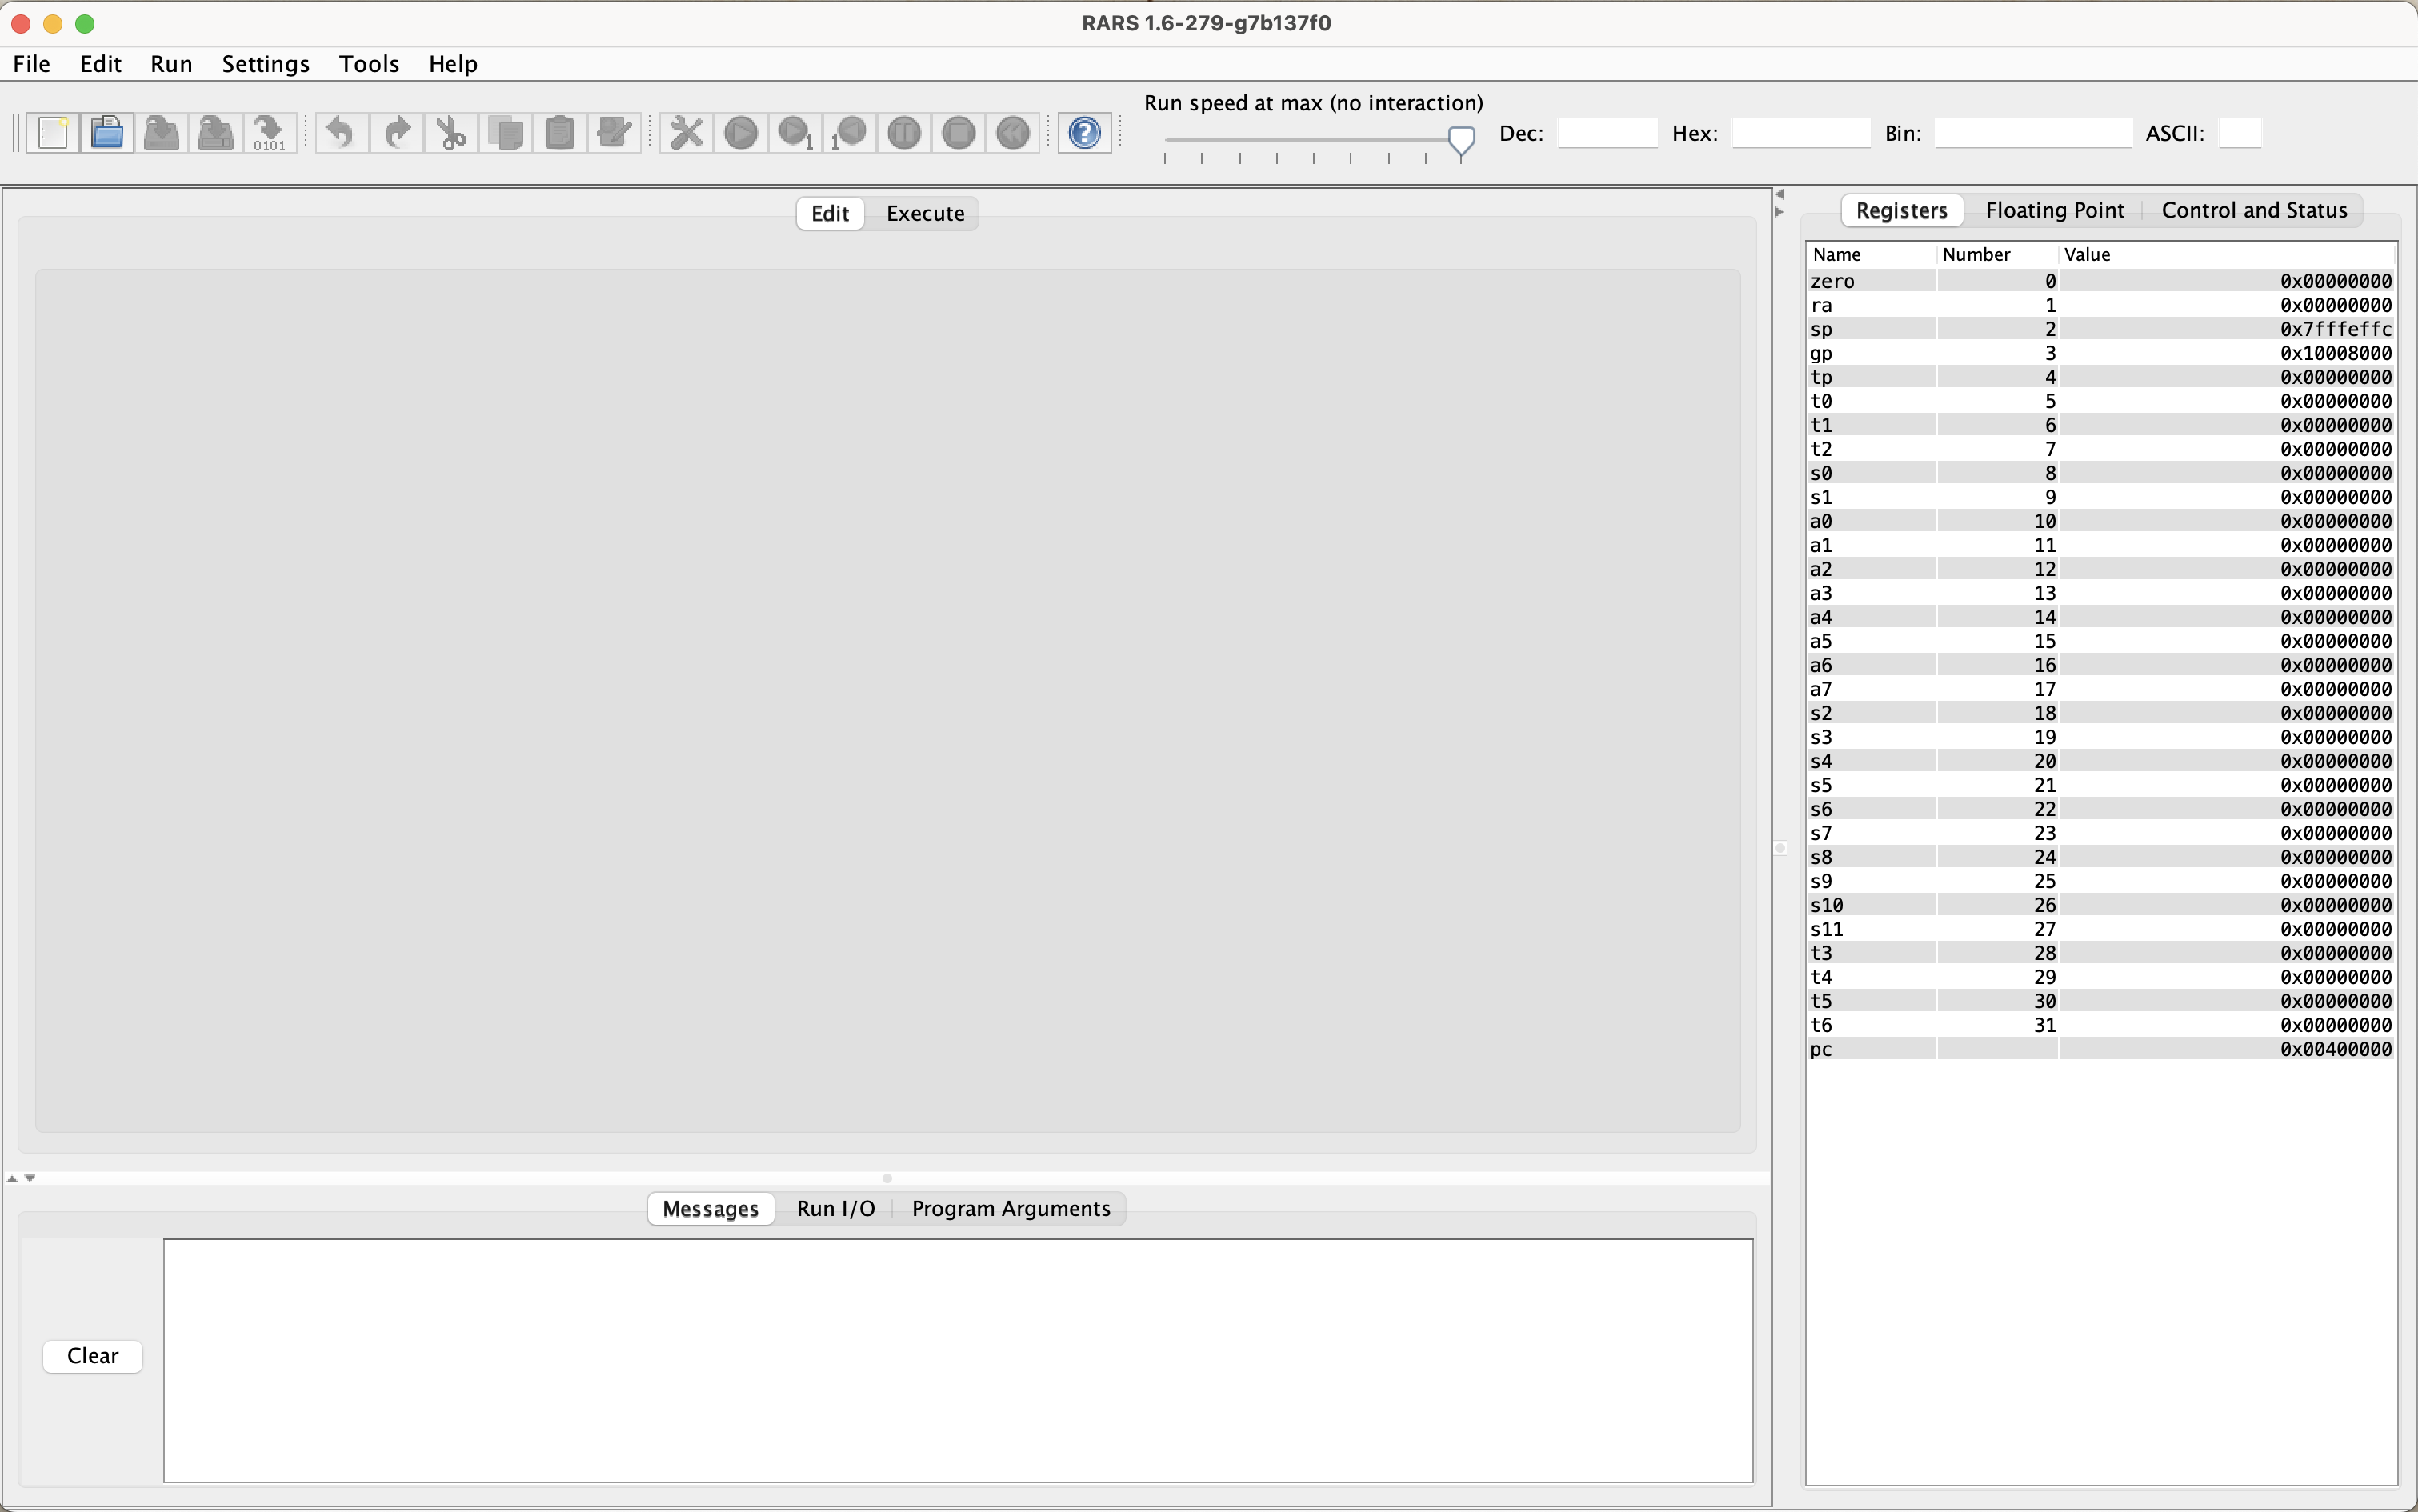
\includegraphics[width=0.85\paperwidth]{rsrcs/0_blankapp.png}}
    %\caption{Recently opened application}
\end{figure}


To open a source file, click on \texttt{Edit > Open ...} and then choose an assembly file.
Remember that RARS assembly files should have the \texttt{.s} extension.

\begin{figure}[H]
    \centering
    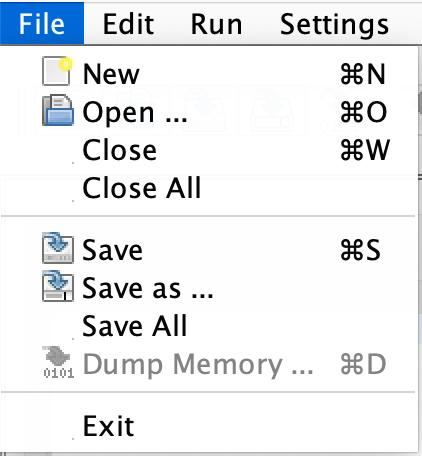
\includegraphics[width=0.35\textwidth]{rsrcs/1_openingfile.png}
    %\caption{1: Openingfile}
\end{figure}

\begin{figure}[H]
    \centering
    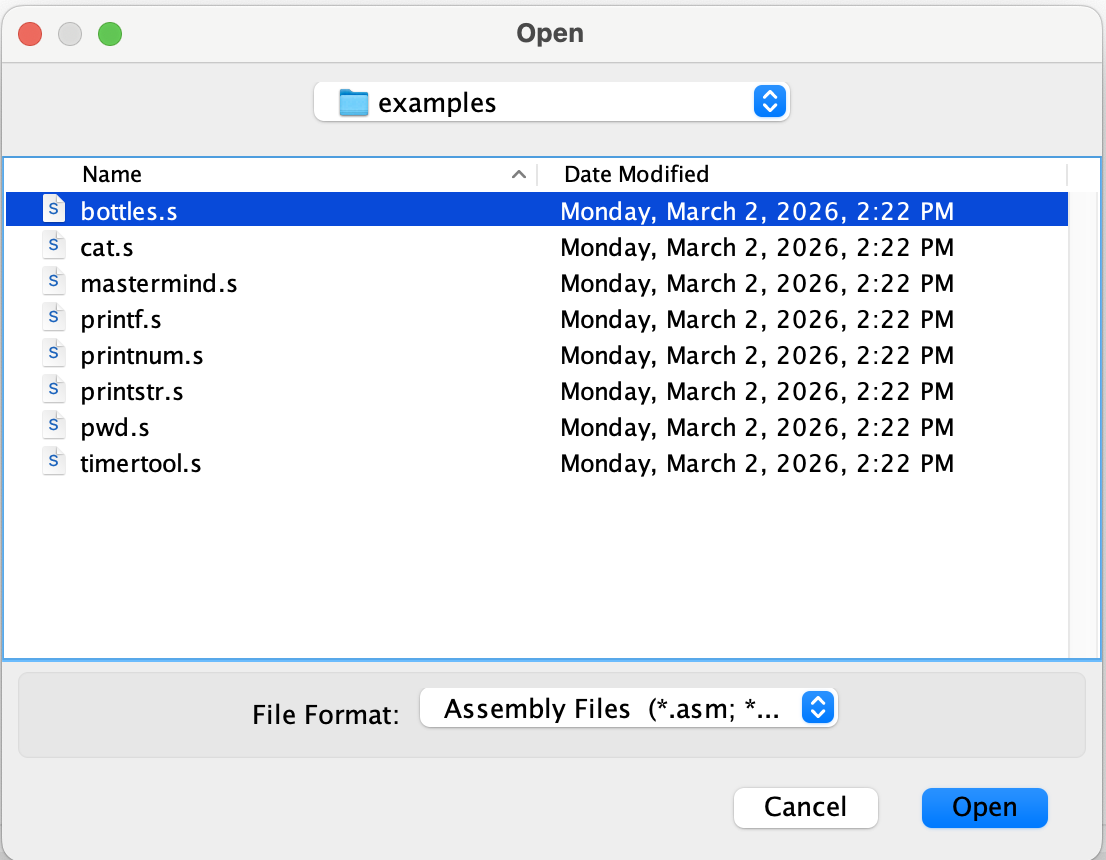
\includegraphics[width=0.8\textwidth]{rsrcs/2_openingfile.png}
    %\caption{2: Openingfile}
\end{figure}


If you see a window like the following image, you should have finalized your basic environment setup.

\begin{figure}[H]
    \centering
    \makebox[\textwidth]{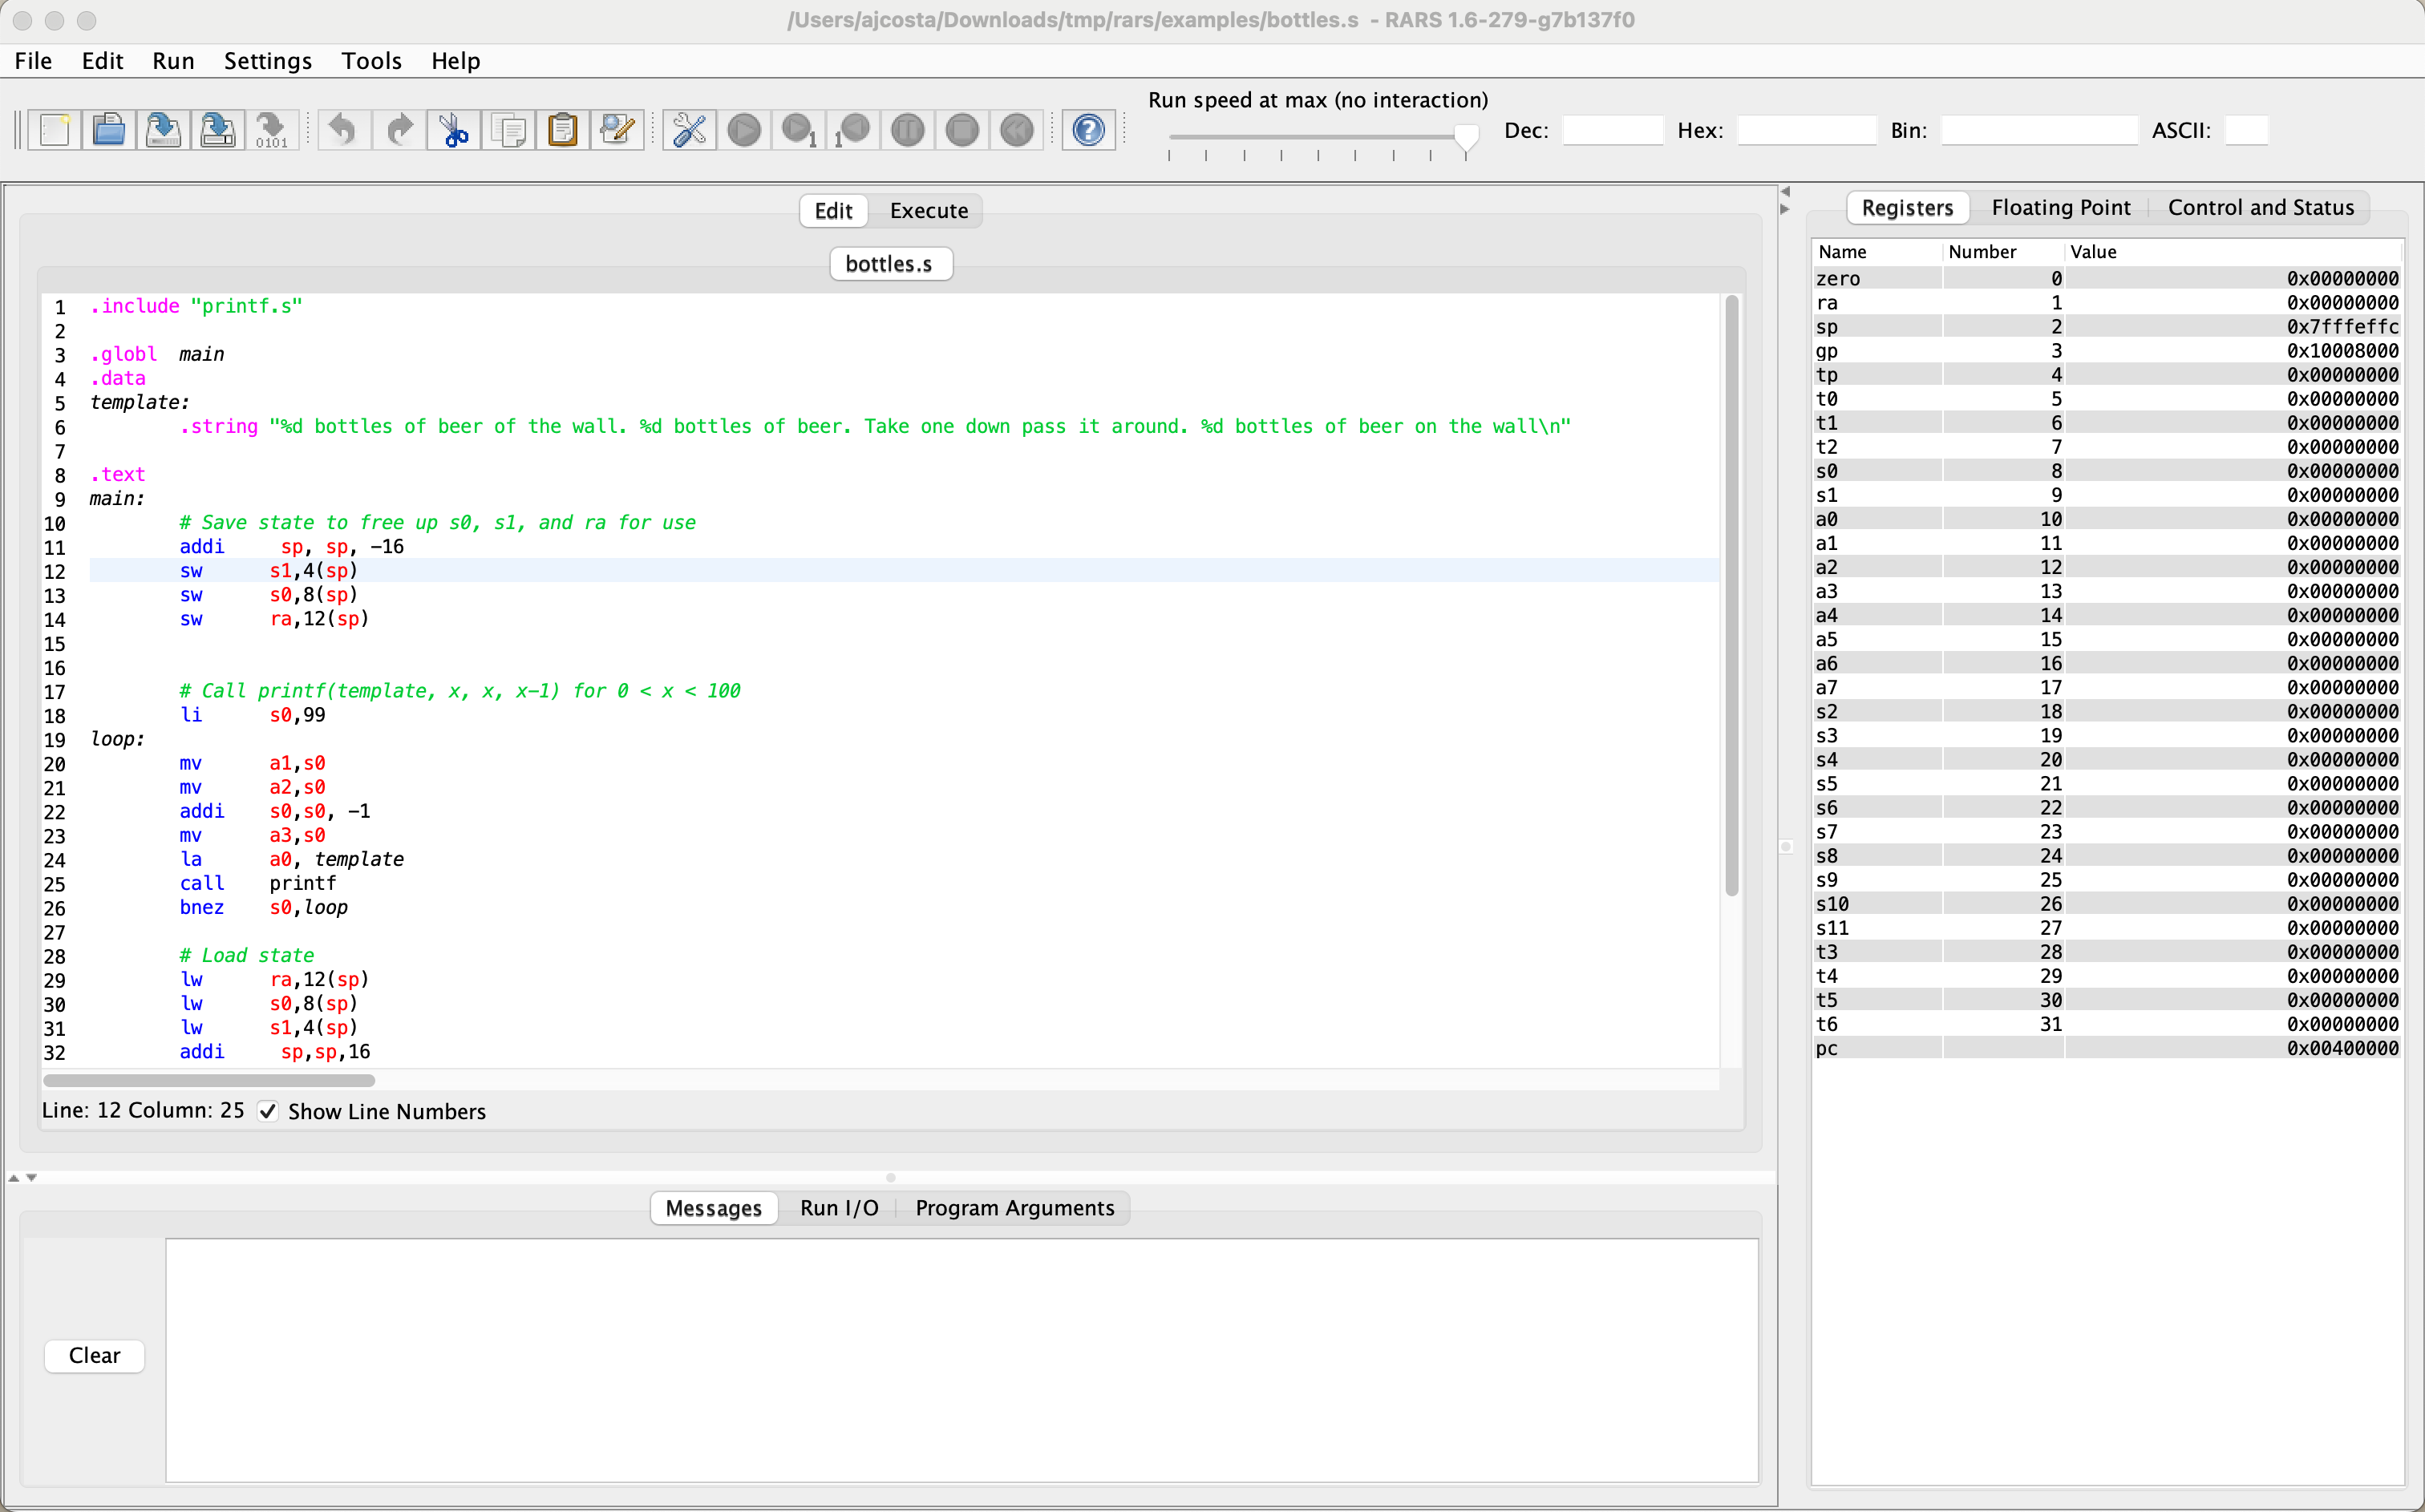
\includegraphics[width=0.85\paperwidth]{rsrcs/3_openingfile.png}}
    %\caption{3: Openingfile}
\end{figure}

\newpage
\section{Running programs}

To run your program, you first need to assemble it to bytecode.
To do that, click the button highlighted in the image below.

\begin{figure}[H]
    \centering
    \makebox[\textwidth]{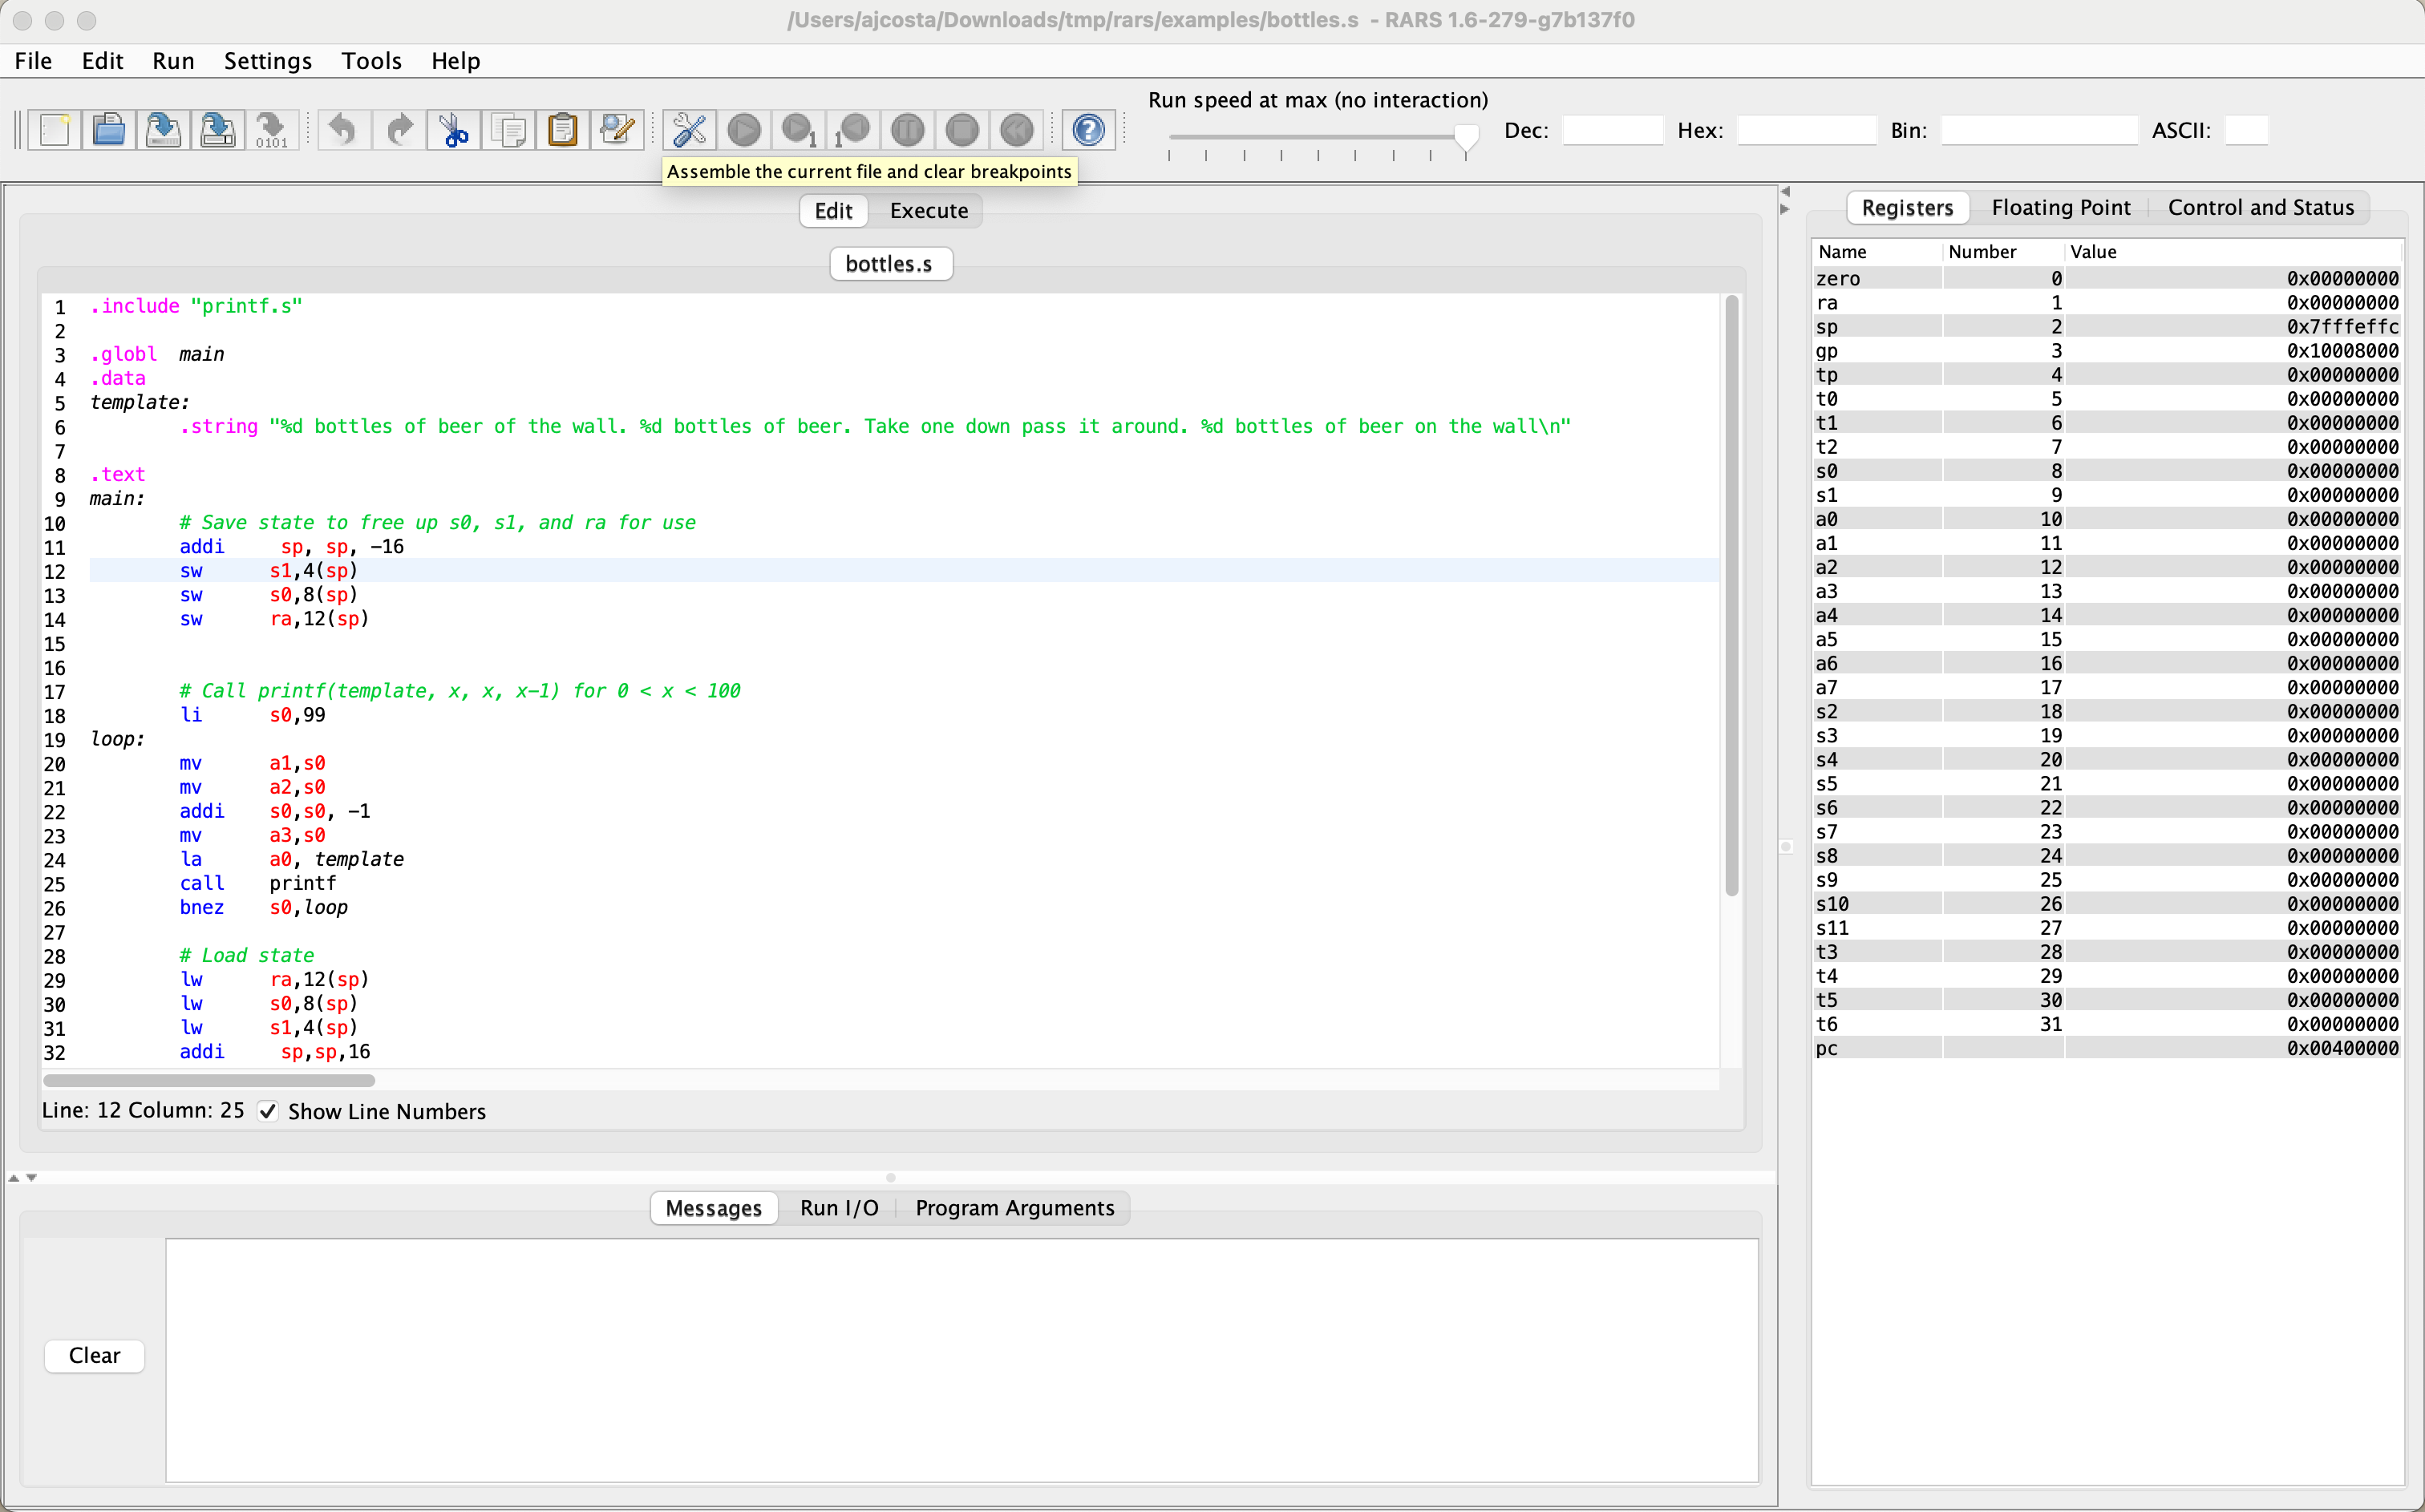
\includegraphics[width=0.85\paperwidth]{rsrcs/4_assemble.png}}
    %\caption{4: Assemble}
\end{figure}

You should be automatically redirected to a window:

\begin{figure}[H]
    \centering
    \makebox[\textwidth]{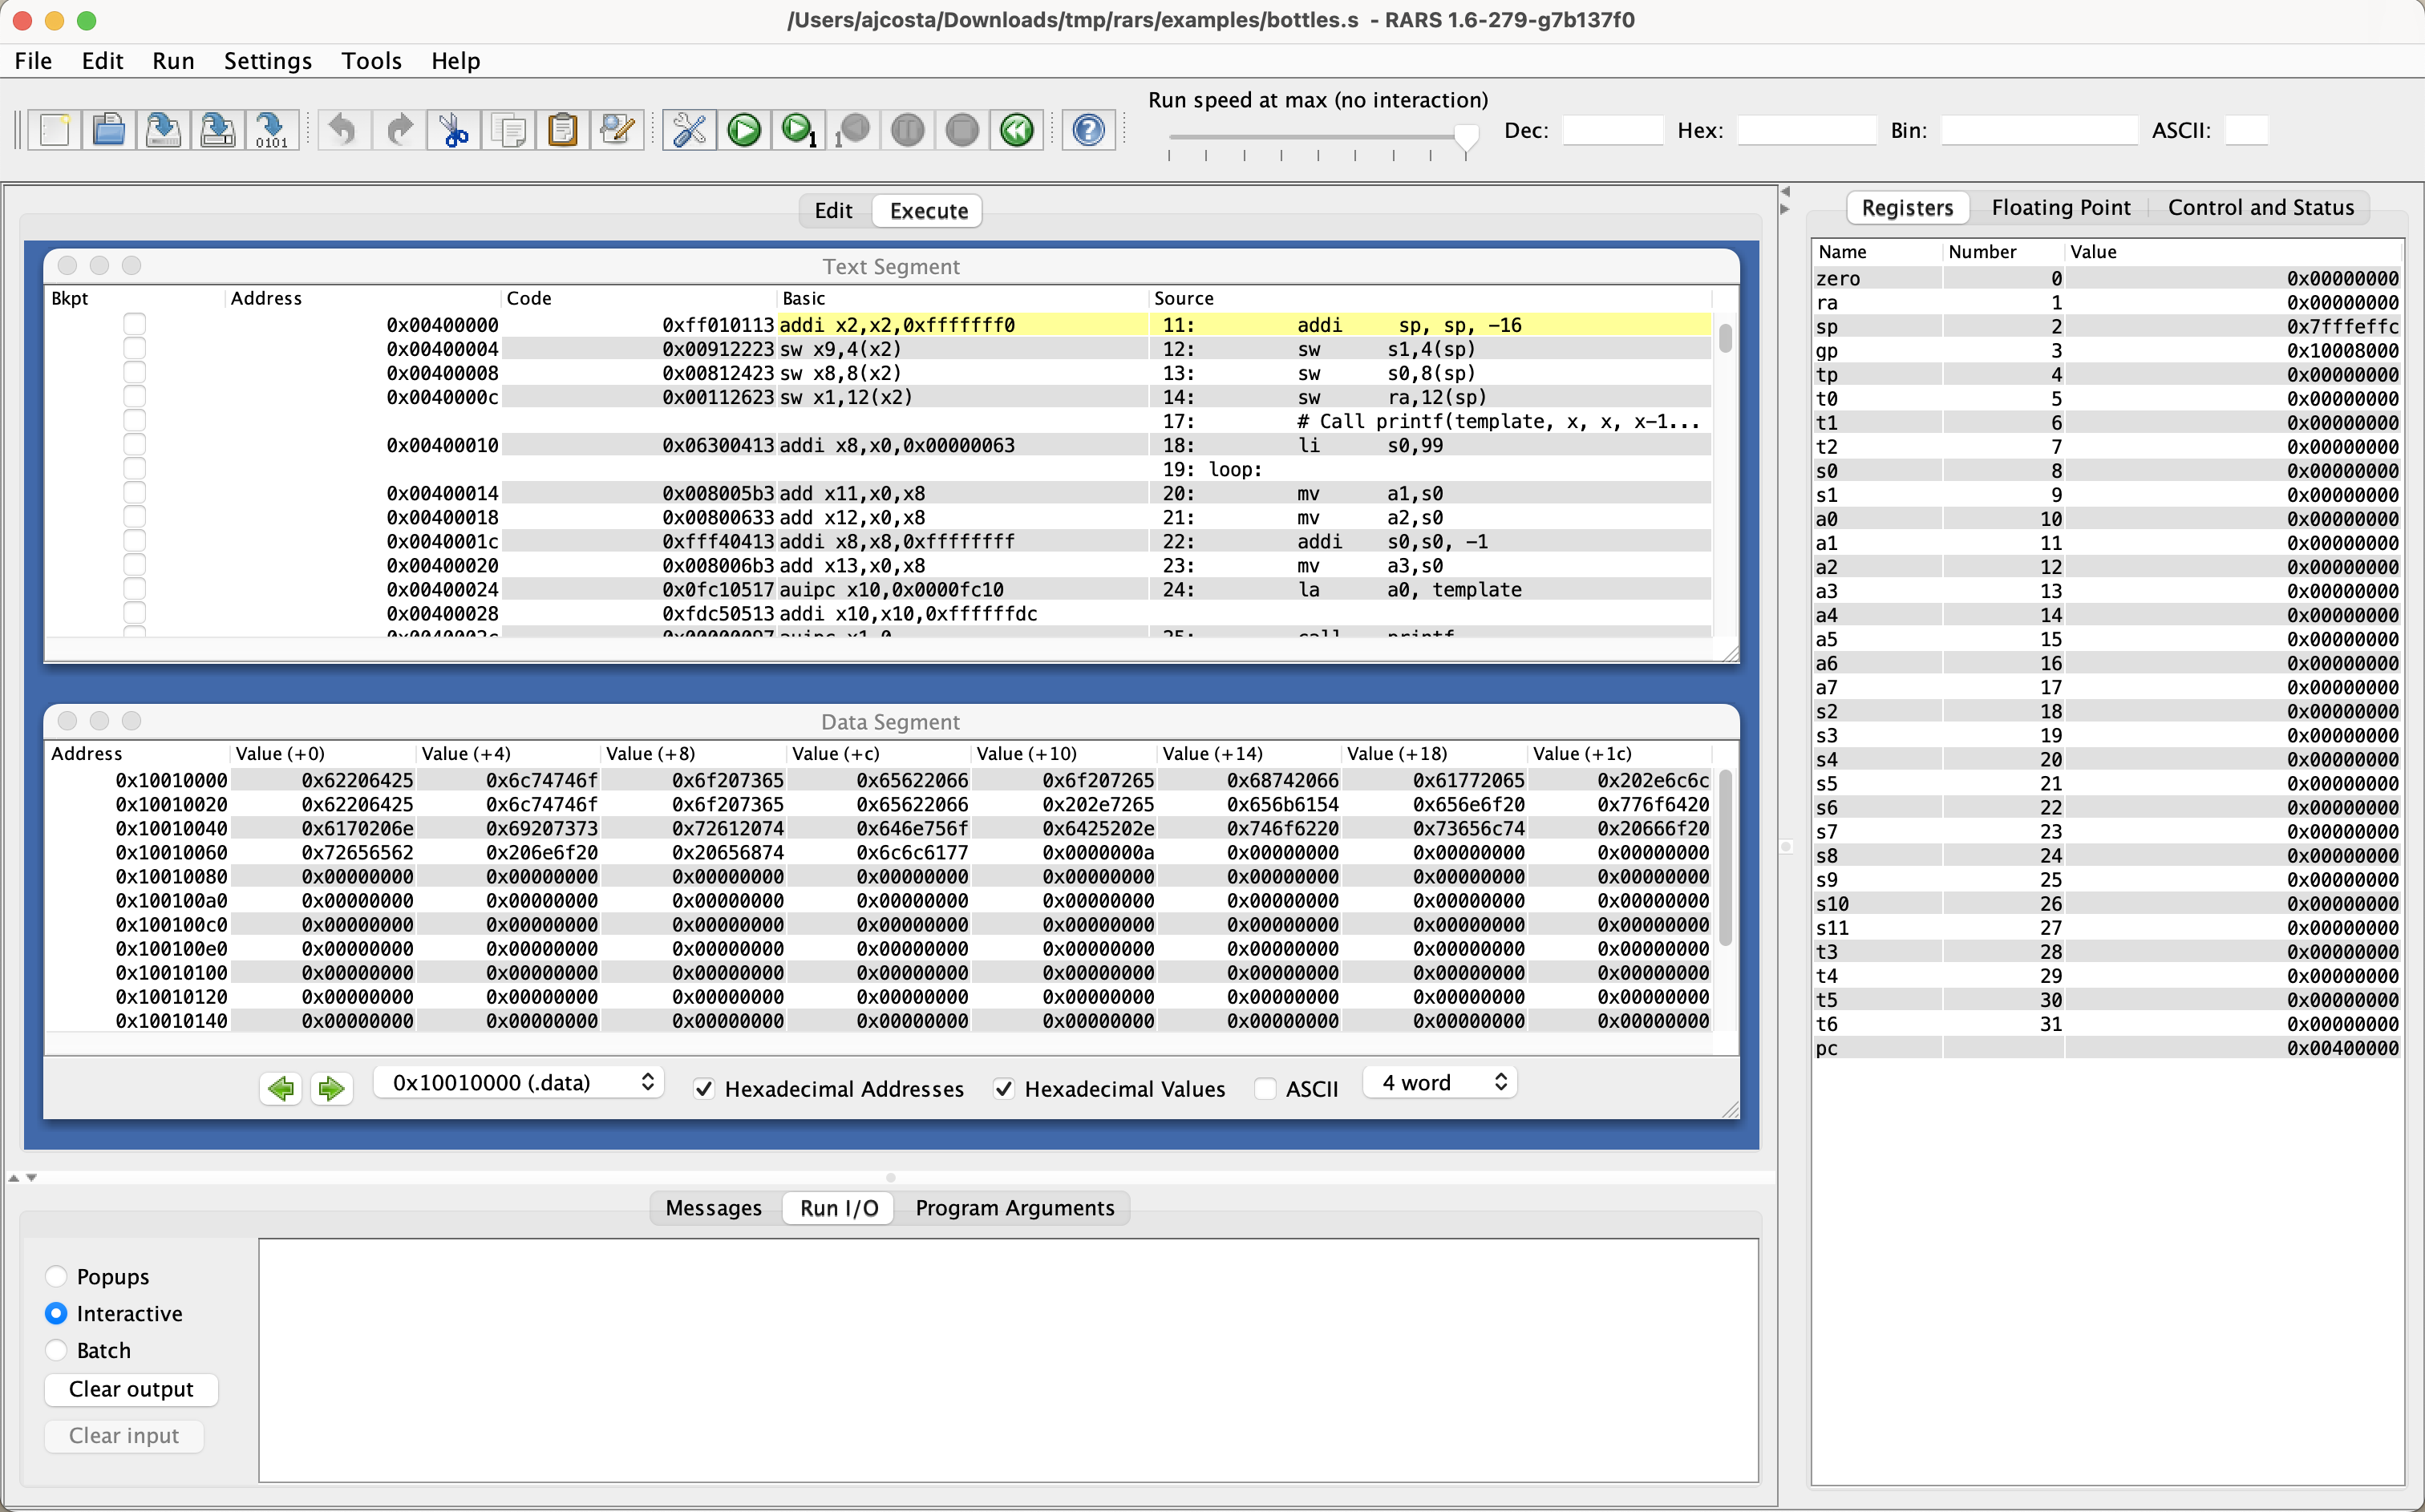
\includegraphics[width=0.85\paperwidth]{rsrcs/5_assemble.png}}
    %\caption{5: Assemble}
\end{figure}

To actually run your program, click the button highlighted below.
This will execute your program to completion.

\begin{figure}[H]
    \centering
    \makebox[\textwidth]{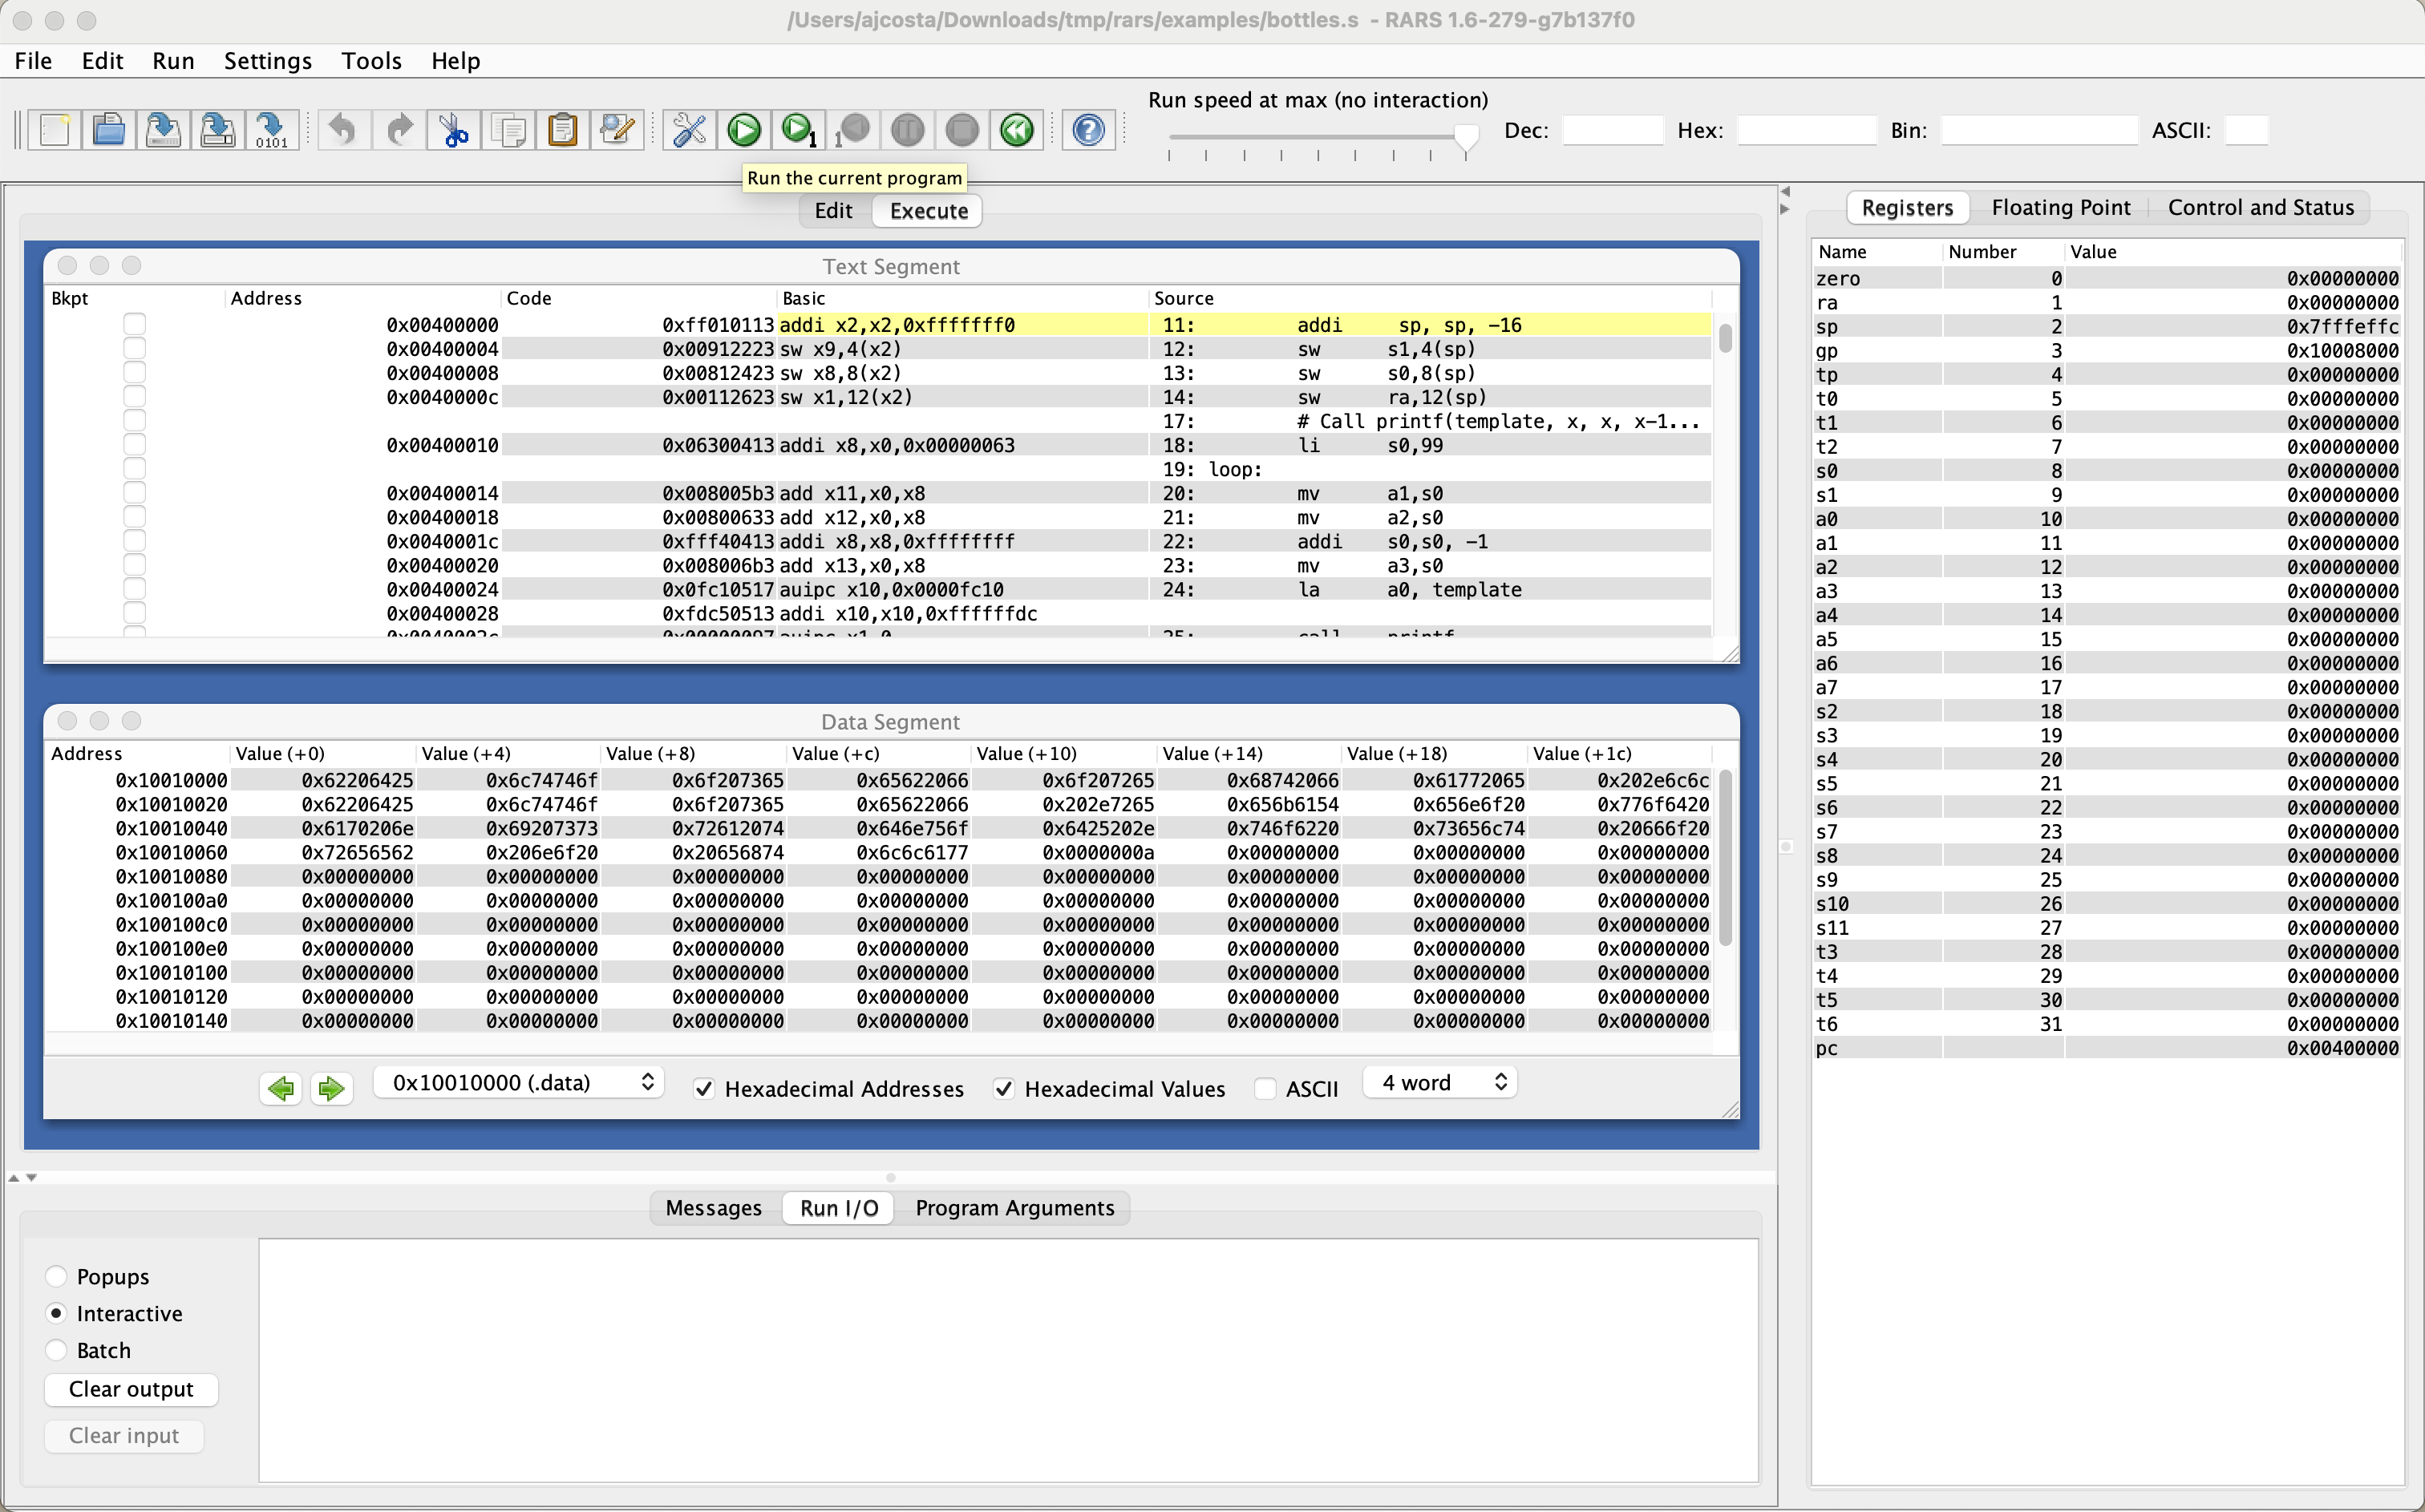
\includegraphics[width=0.85\paperwidth]{rsrcs/6_execute.png}}
    %\caption{6: Execute}
\end{figure}

You can see the (printed) output in the \texttt{Run I/O} box.

\begin{figure}[H]
    \centering
    \makebox[\textwidth]{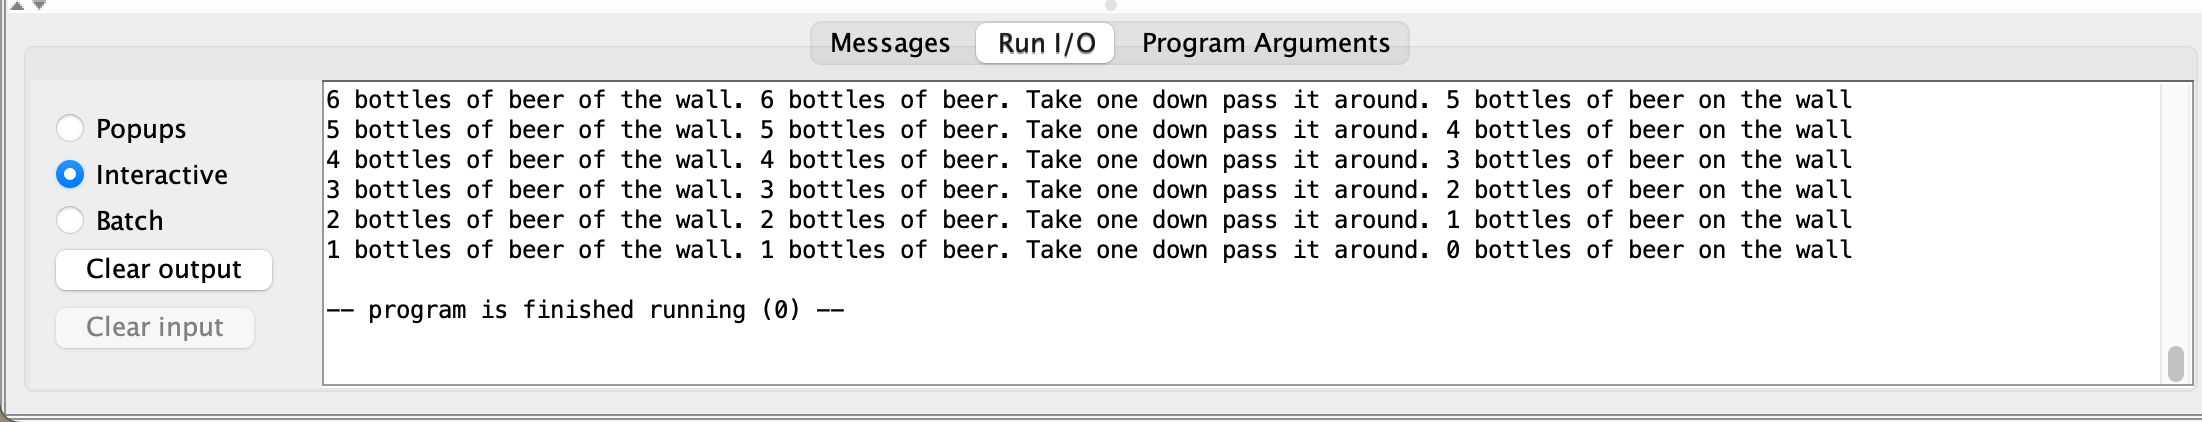
\includegraphics[width=0.85\paperwidth]{rsrcs/7_execute.png}}
    %\caption{7: Execute}
\end{figure}

The box at the right of the window shows the values that each registers hold.
By default it shows general purpose registers, but you can also look at other registers by clicking \texttt{Control and Status}/

\begin{figure}[H]
    \centering
    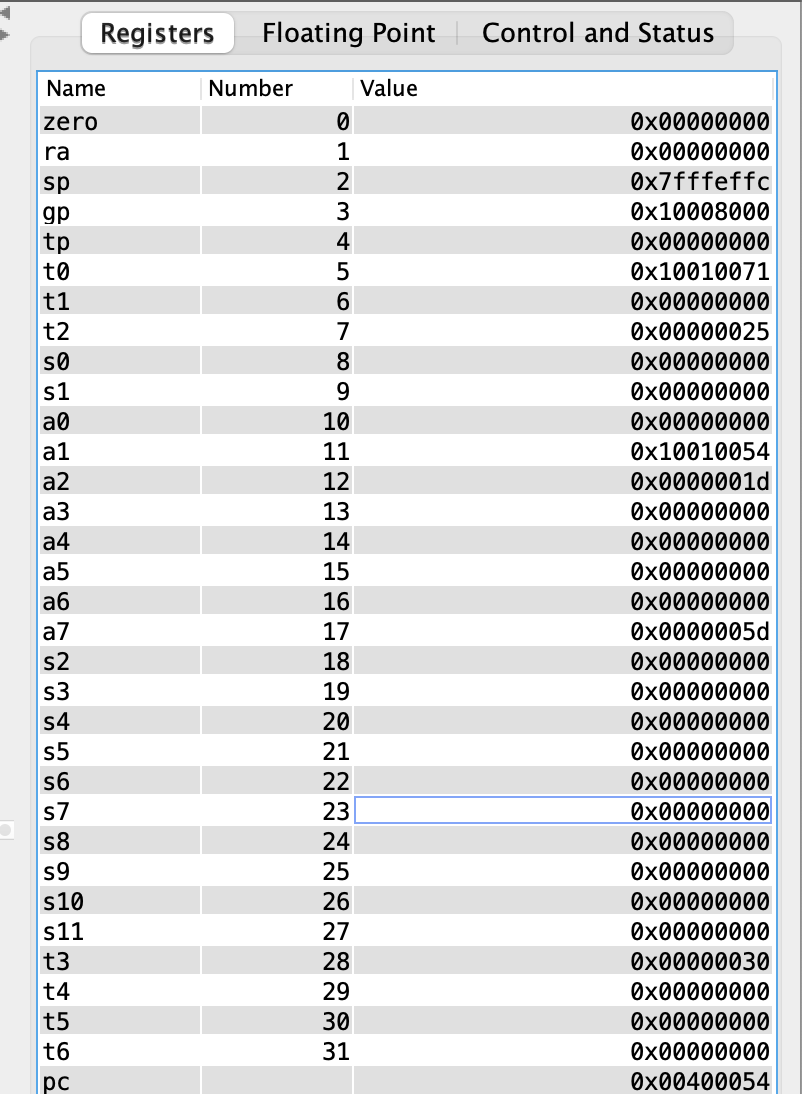
\includegraphics[width=0.5\textwidth]{rsrcs/8_execute.png}
    %\caption{8: Execute}
\end{figure}

To run your program again, RARS requries that you rewind each instruction that was previously executed.
To rewind all instructions in one go, click the \textsc{Reset memory and register} button.

\begin{figure}[H]
    \centering
    \makebox[\textwidth]{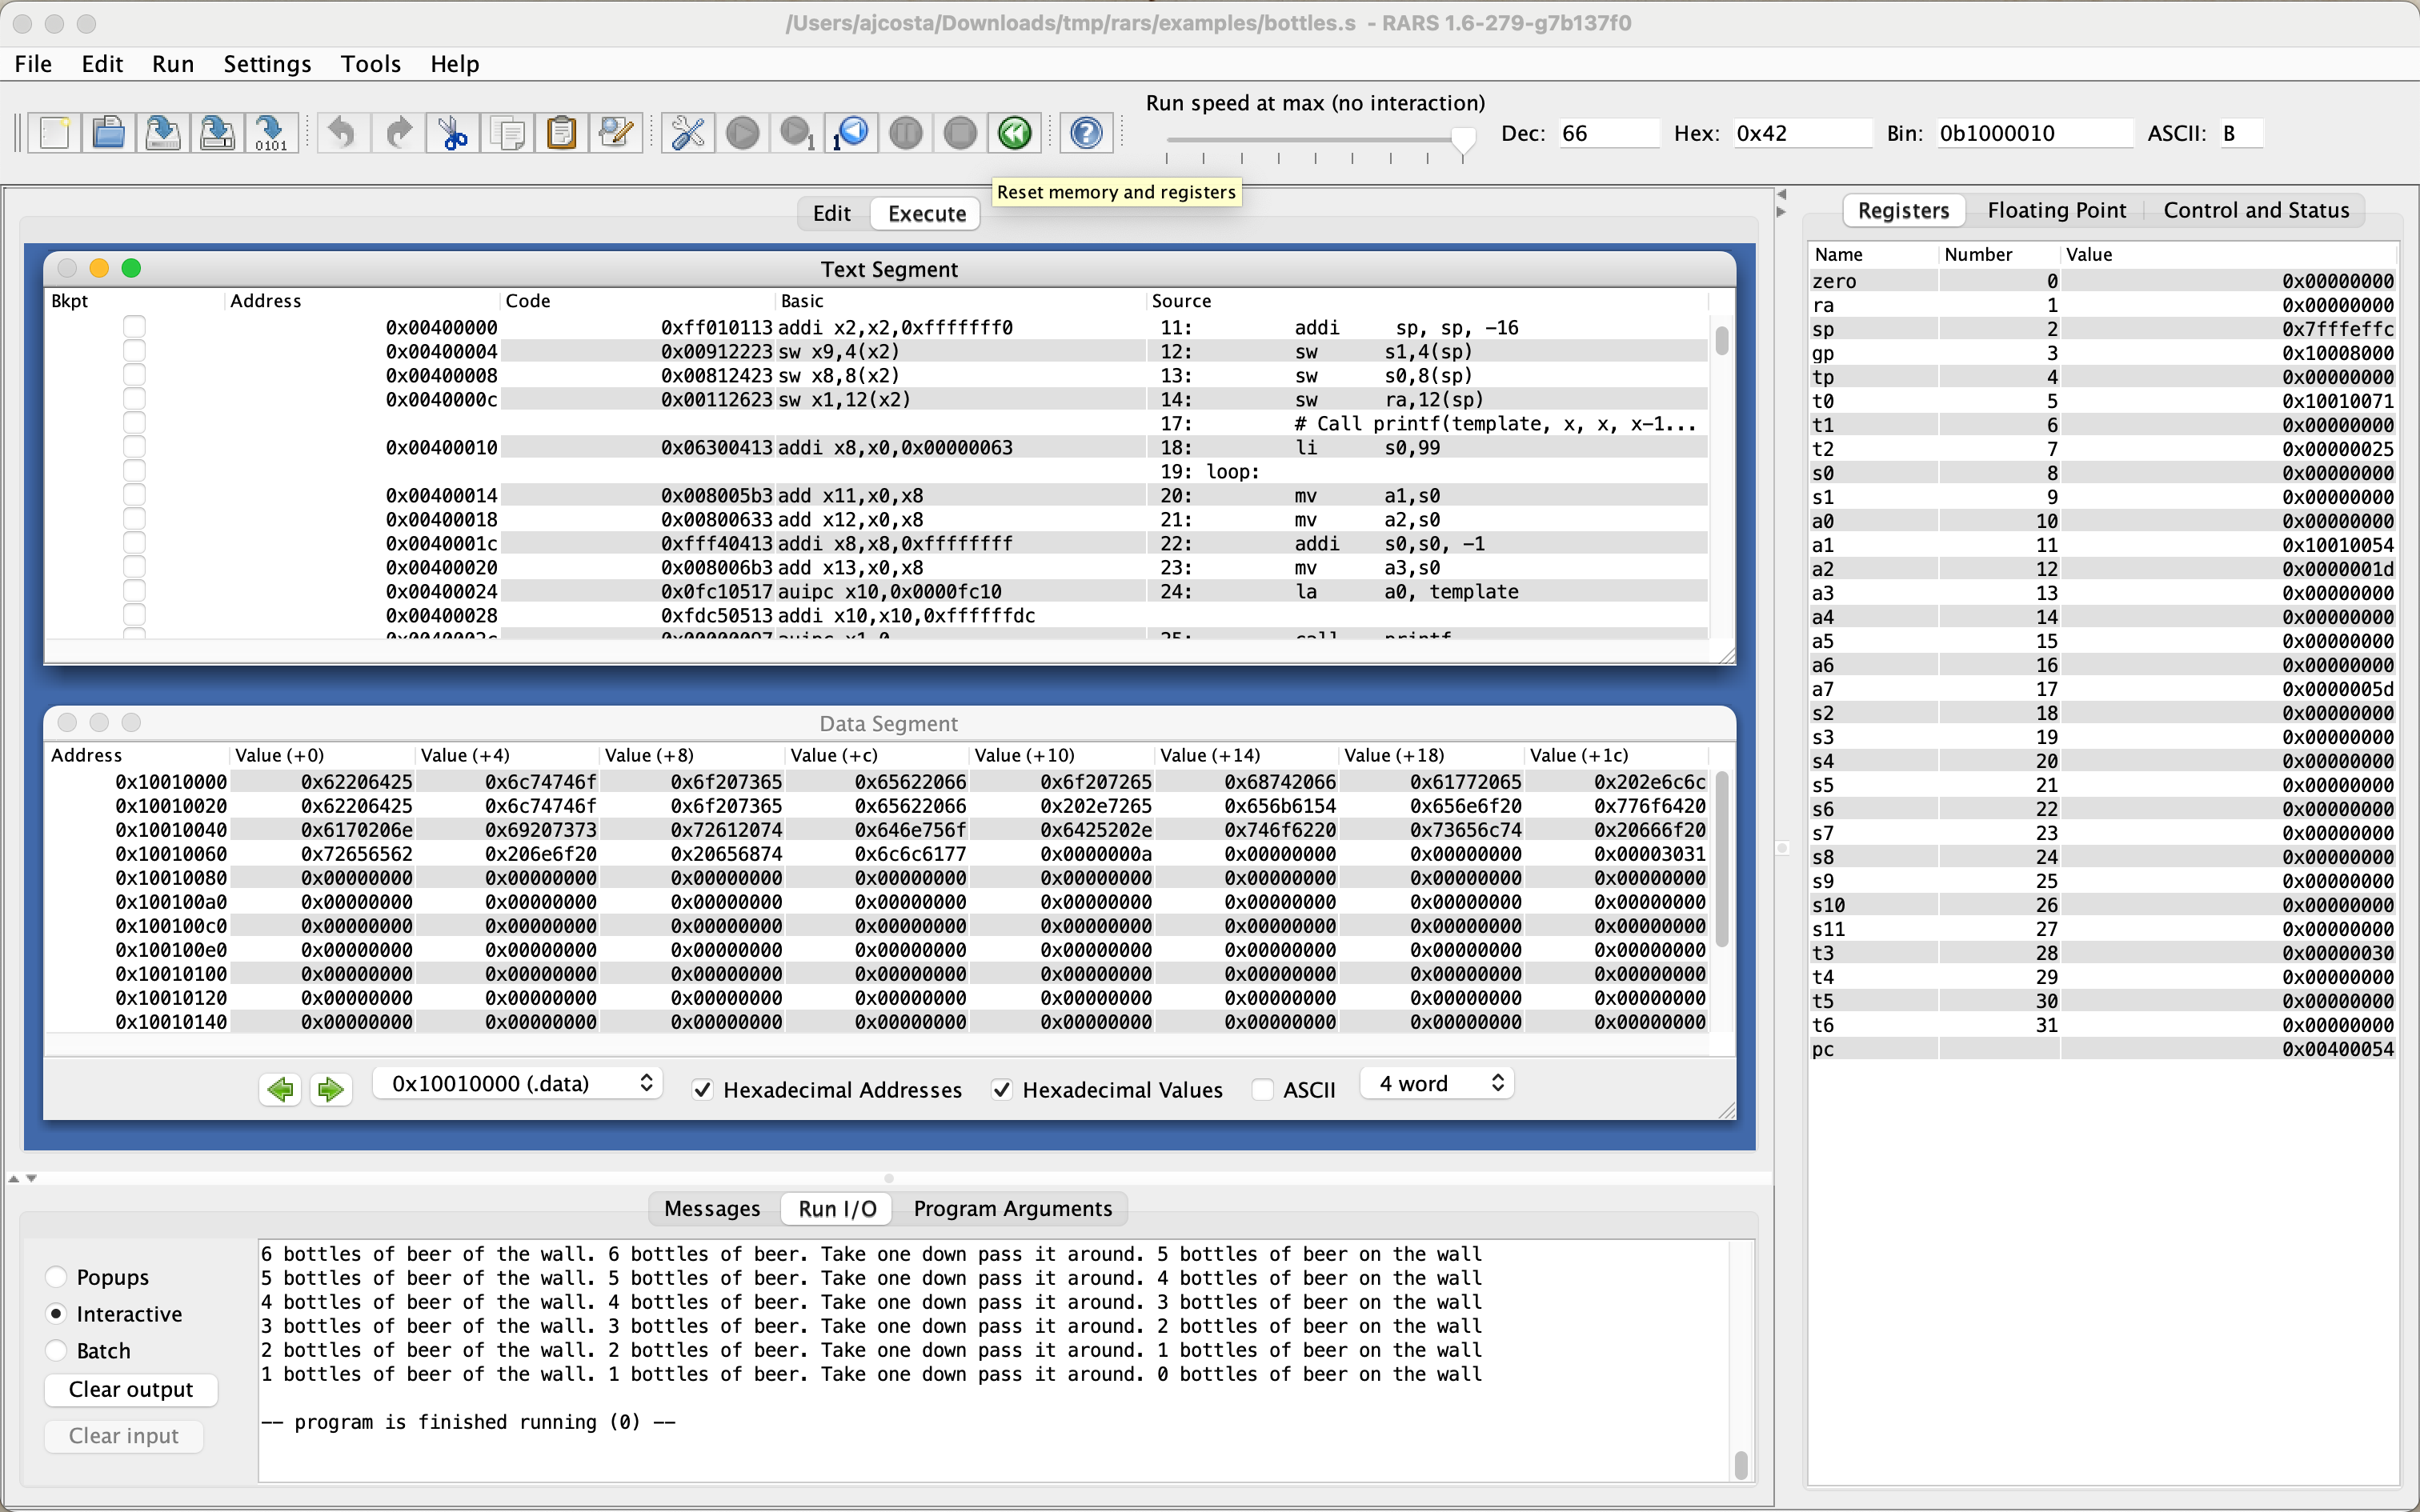
\includegraphics[width=0.85\paperwidth]{rsrcs/9_execute.png}}
    %\caption{9: Execute}
\end{figure}

\section{Debugging}

To aid in debugging your program, RARS allows you to execute one instruction at a time.
To do that, click the \texttt{Run one step at a time} button.

\begin{figure}[H]
    \centering
    \makebox[\textwidth]{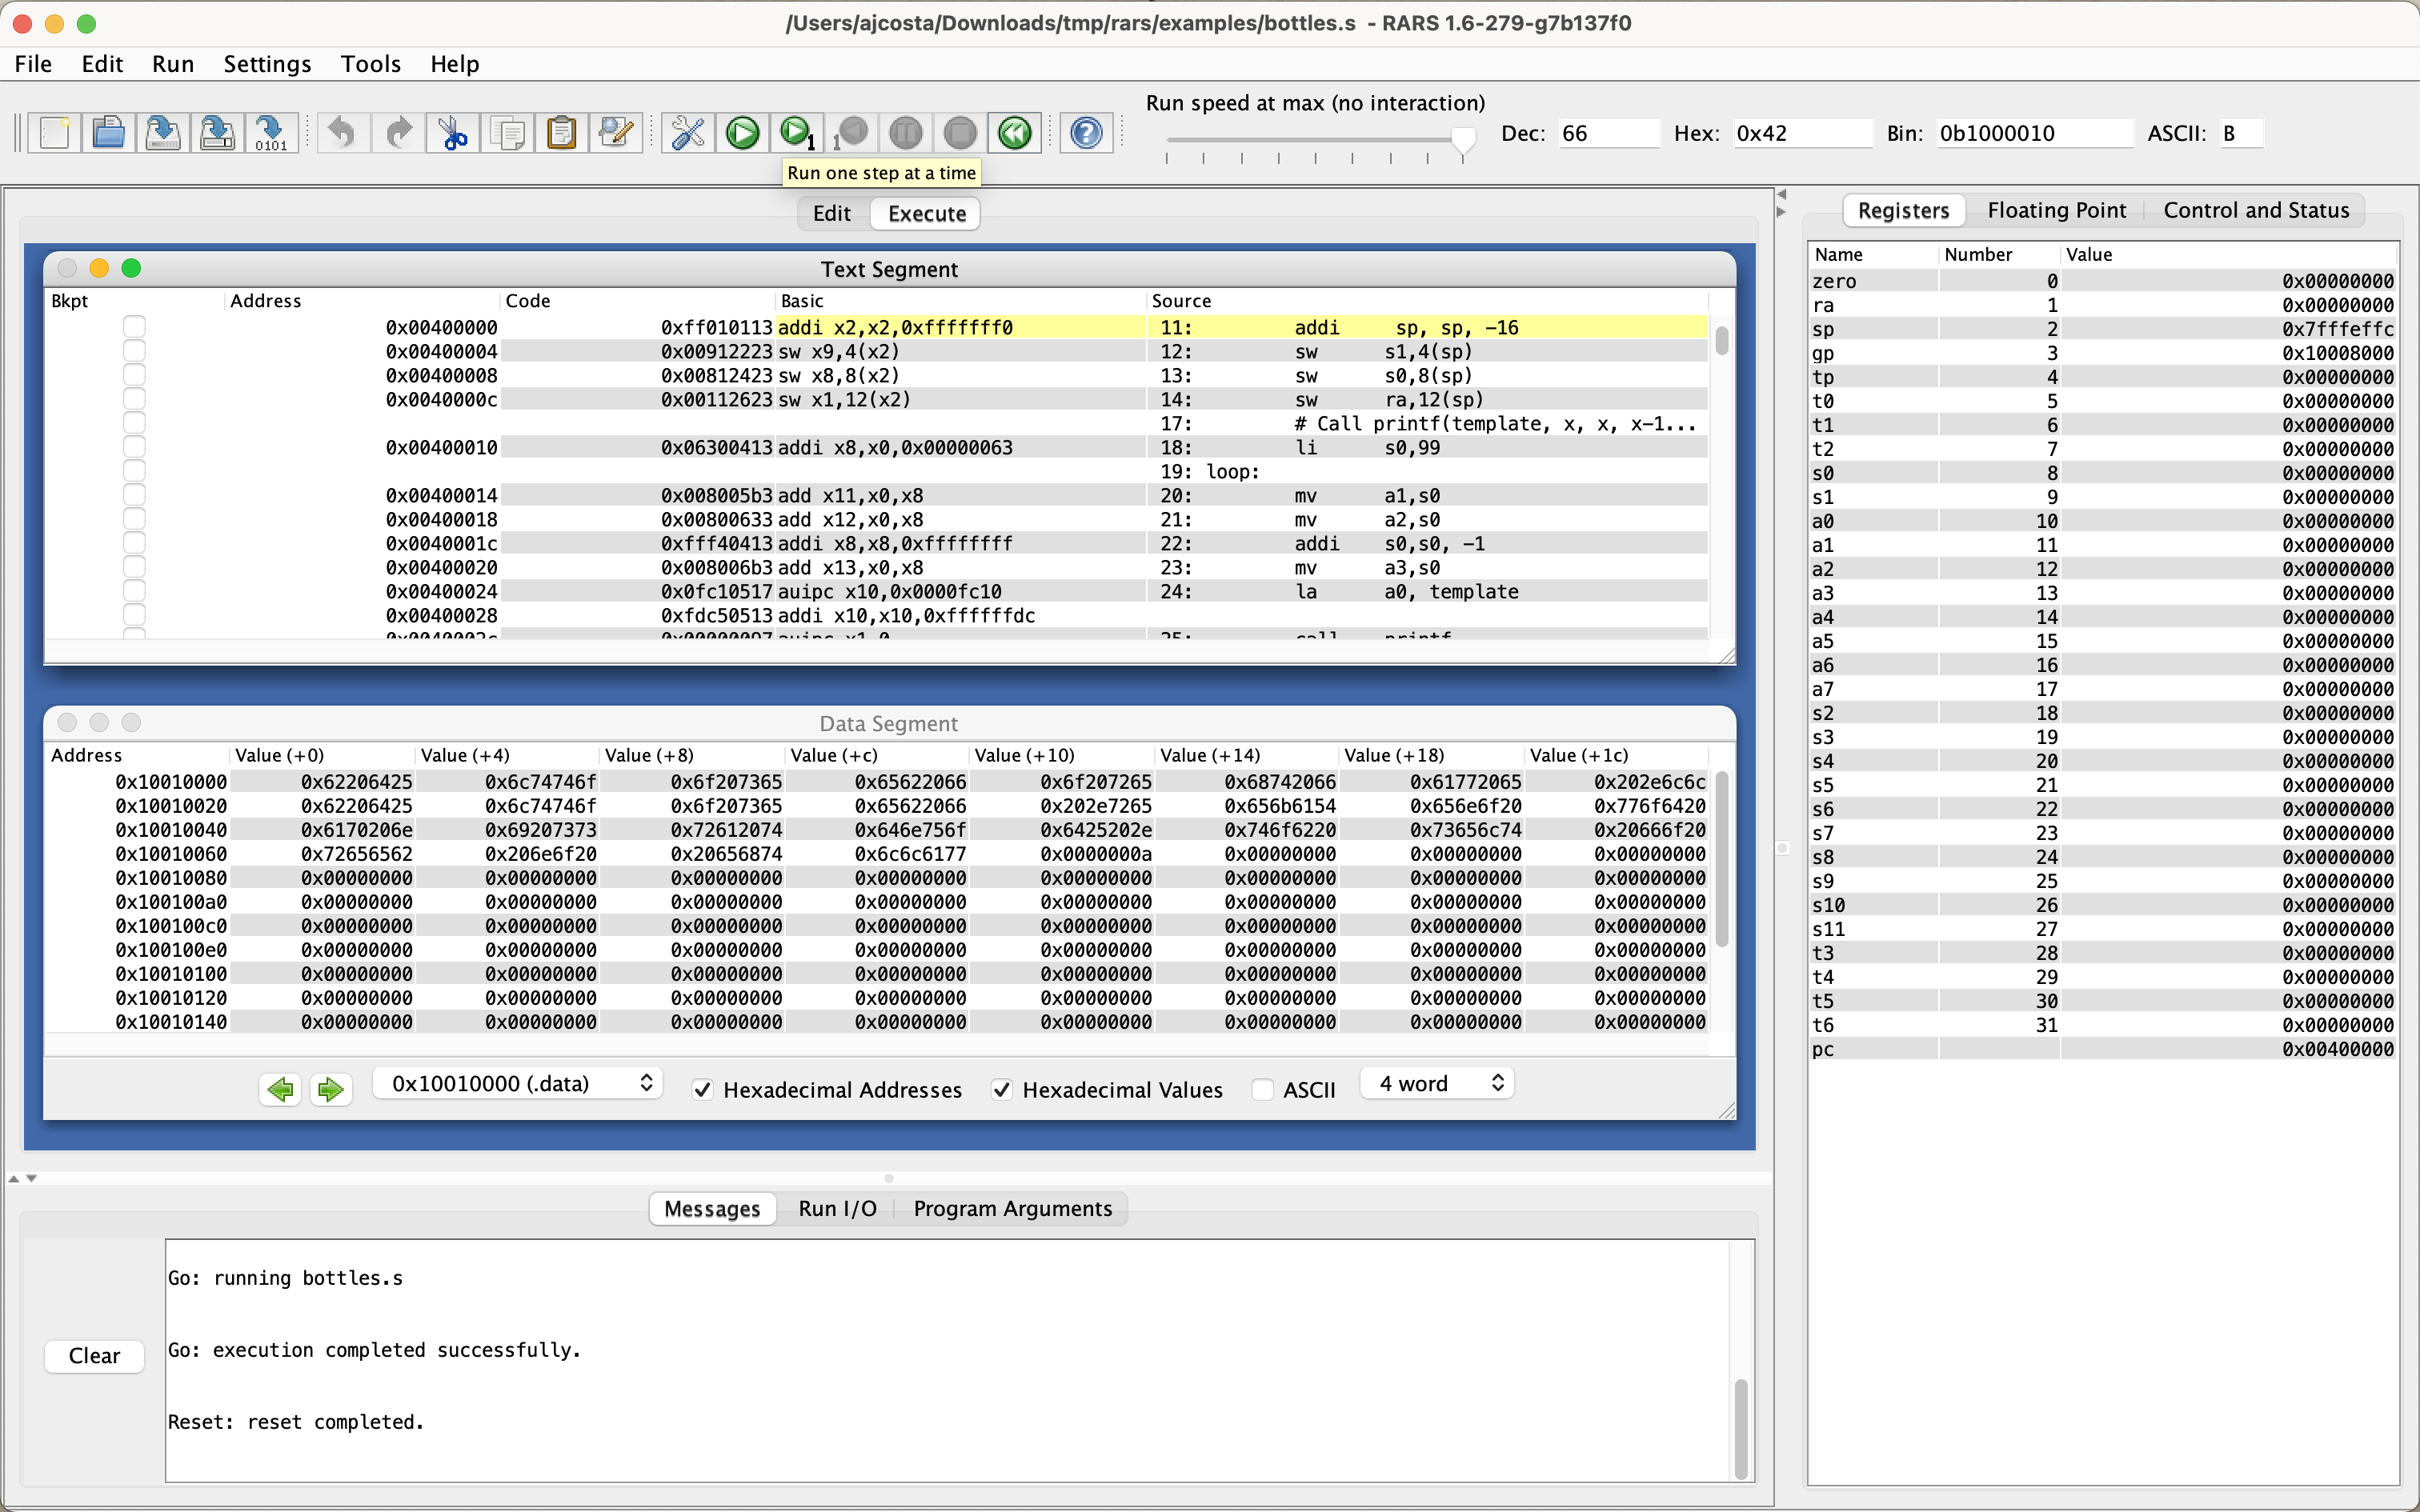
\includegraphics[width=0.85\paperwidth]{rsrcs/10_debug.png}}
    %\caption{10: Debug}
\end{figure}

RARS is really friendly, so it will highlight which registers were changed by each instruction!
The following image shows RARS after executing the \texttt{add x12, x0, 0x8} instruction.
The registers highlighted in {\textcolor{blue}{blue}} show the input registers (\texttt{x0} and
\texttt{x8} in this case), while the register in {\textcolor{red}{red}} show the output register (\texttt{x12}).

\begin{figure}[H]
    \centering
    \makebox[\textwidth]{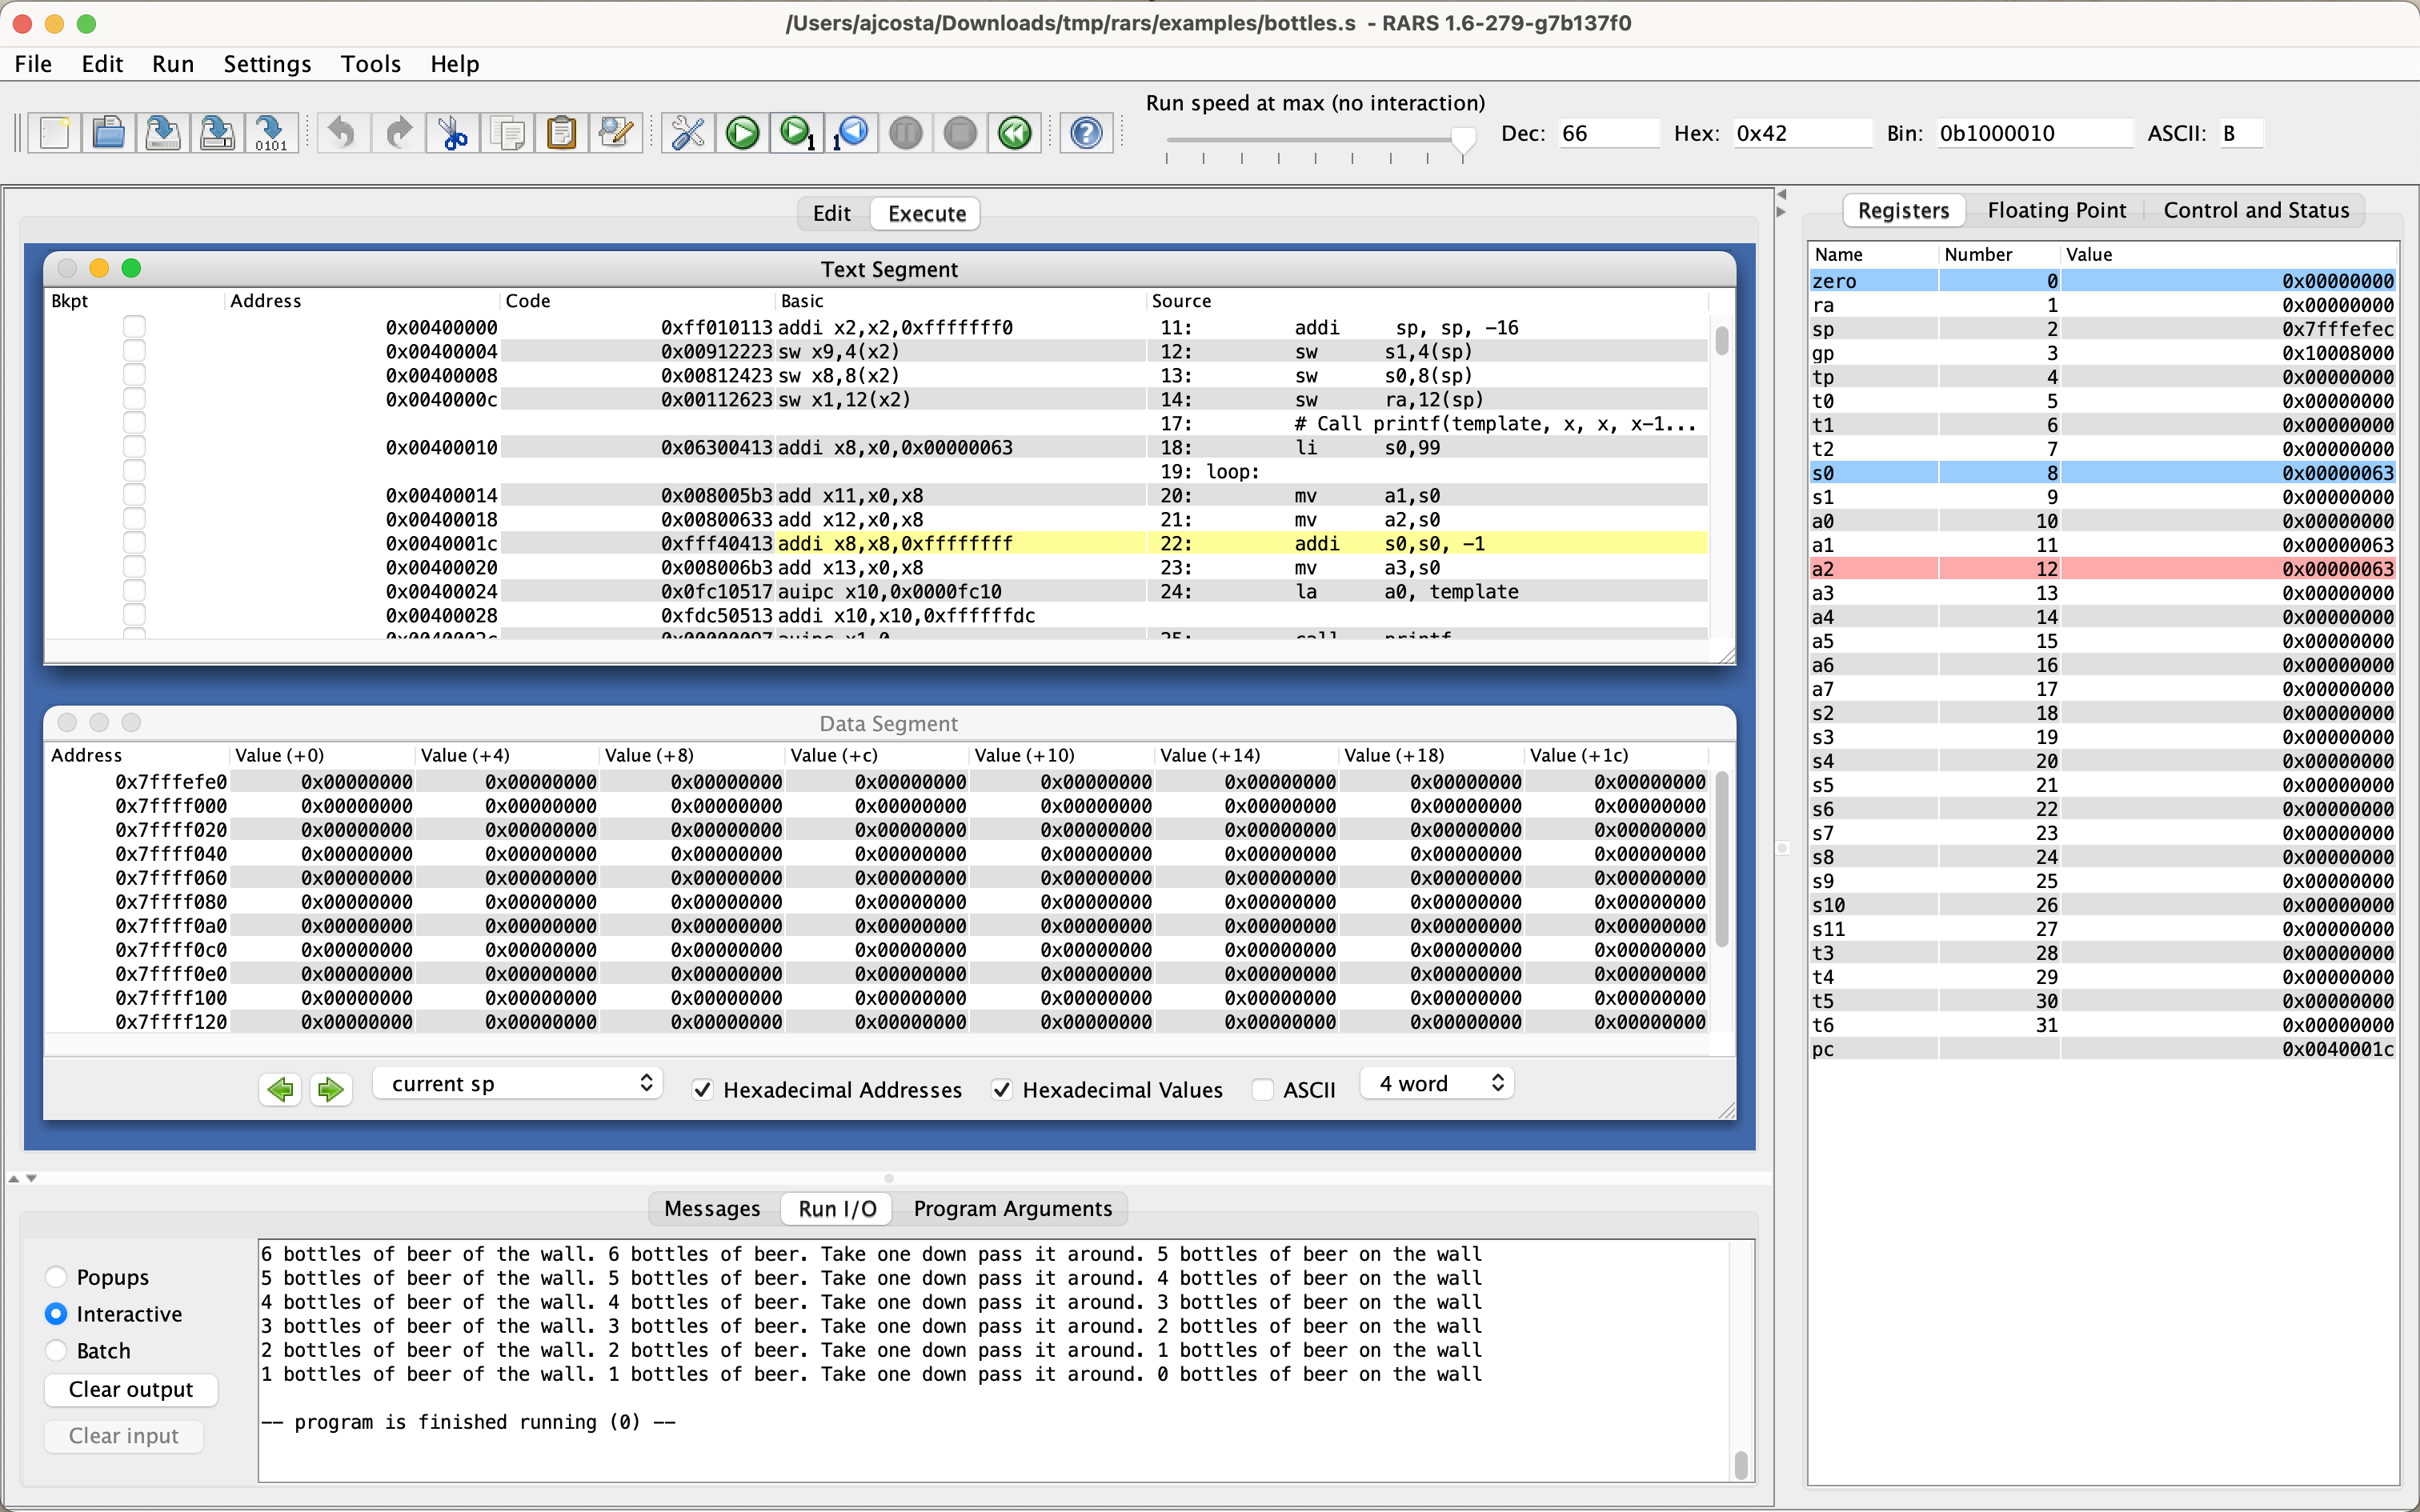
\includegraphics[width=0.85\paperwidth]{rsrcs/11_debug.png}}
    %\caption{11: Debug}
\end{figure}

Like I said, RARS is \textbf{really} friendly, so it allows you to undo an instruction!
Just click the \texttt{Undo the last step} button.

\begin{figure}[H]
    \centering
    \makebox[\textwidth]{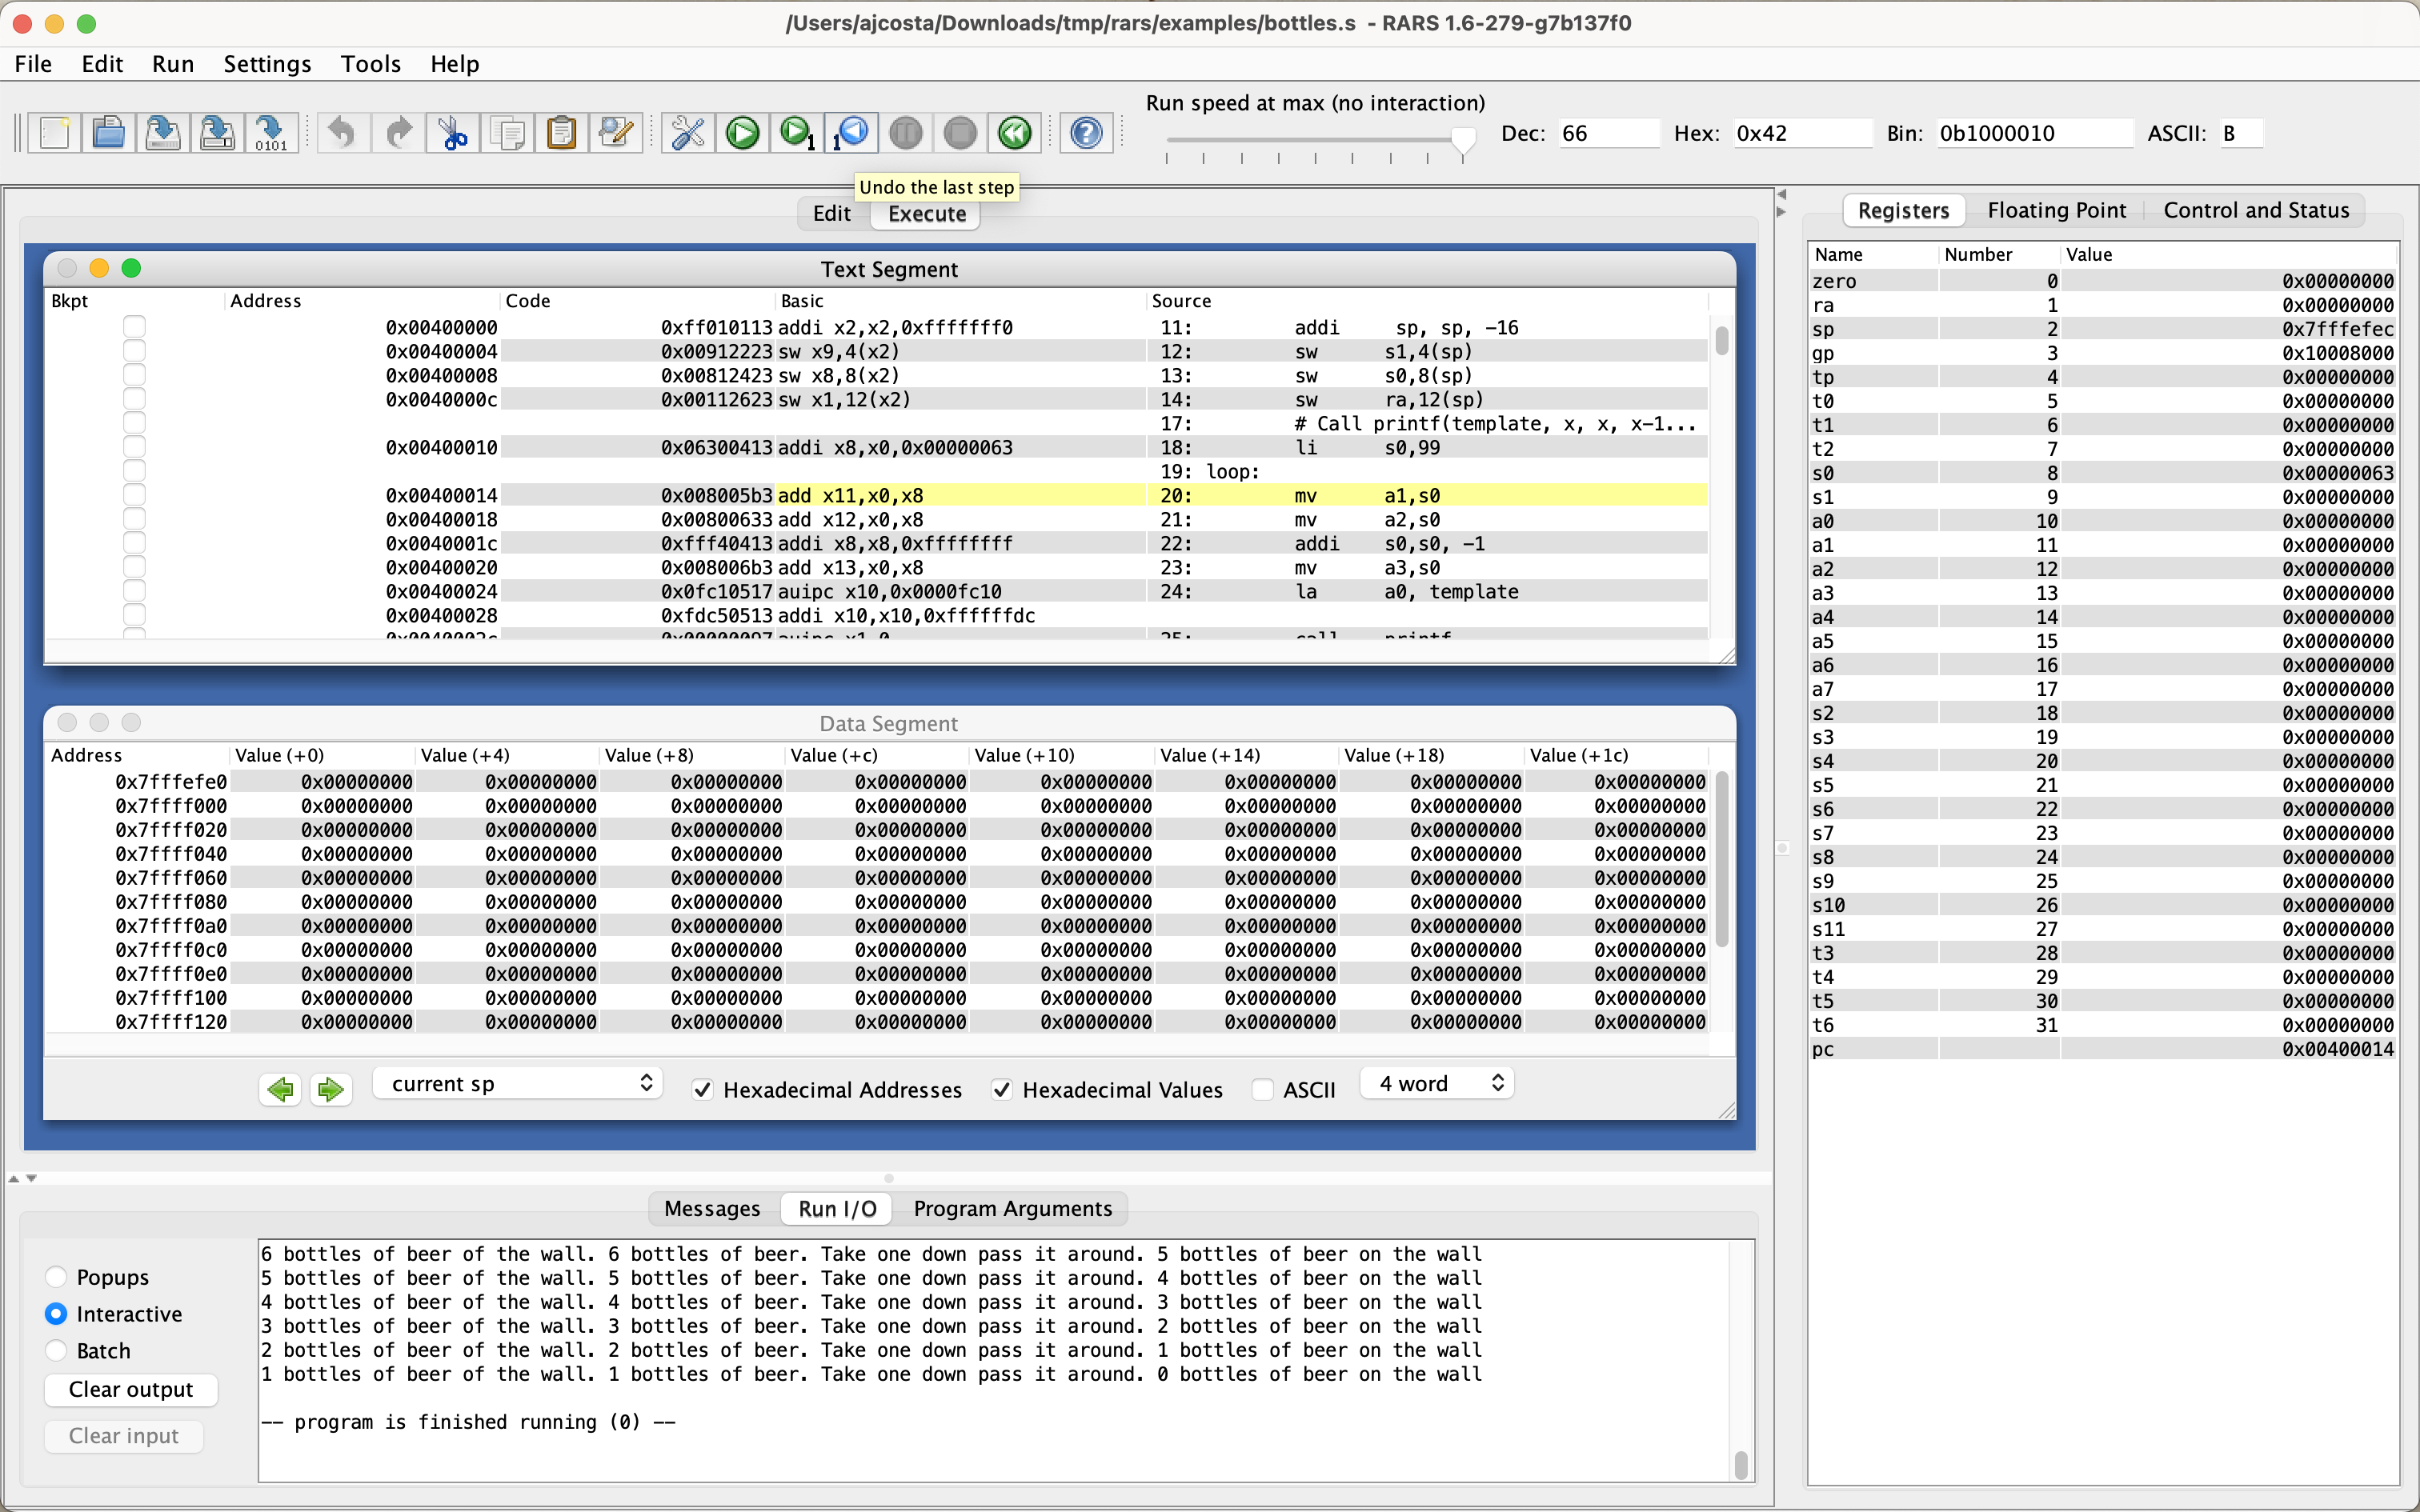
\includegraphics[width=0.85\paperwidth]{rsrcs/12_debug.png}}
    %\caption{12: Debug}
\end{figure}

Finally, to help you look values in different representations, RARS has this box that allows you to do conversions easily.

\begin{figure}[H]
    \centering
    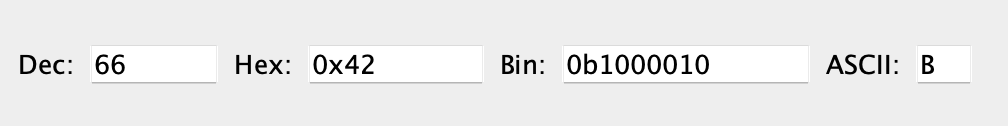
\includegraphics[width=0.65\paperwidth]{rsrcs/13_debug.png}
    %\caption{13: Debug}
\end{figure}


Finally, you can also run your programs directly in the terminal!
Here is an example:
\inputterminal{rsrcs/1_runterminal.txt}

\section{Documentation}

If you're in need of some help, click Help!

\begin{figure}[H]
    \centering
    \makebox[\textwidth]{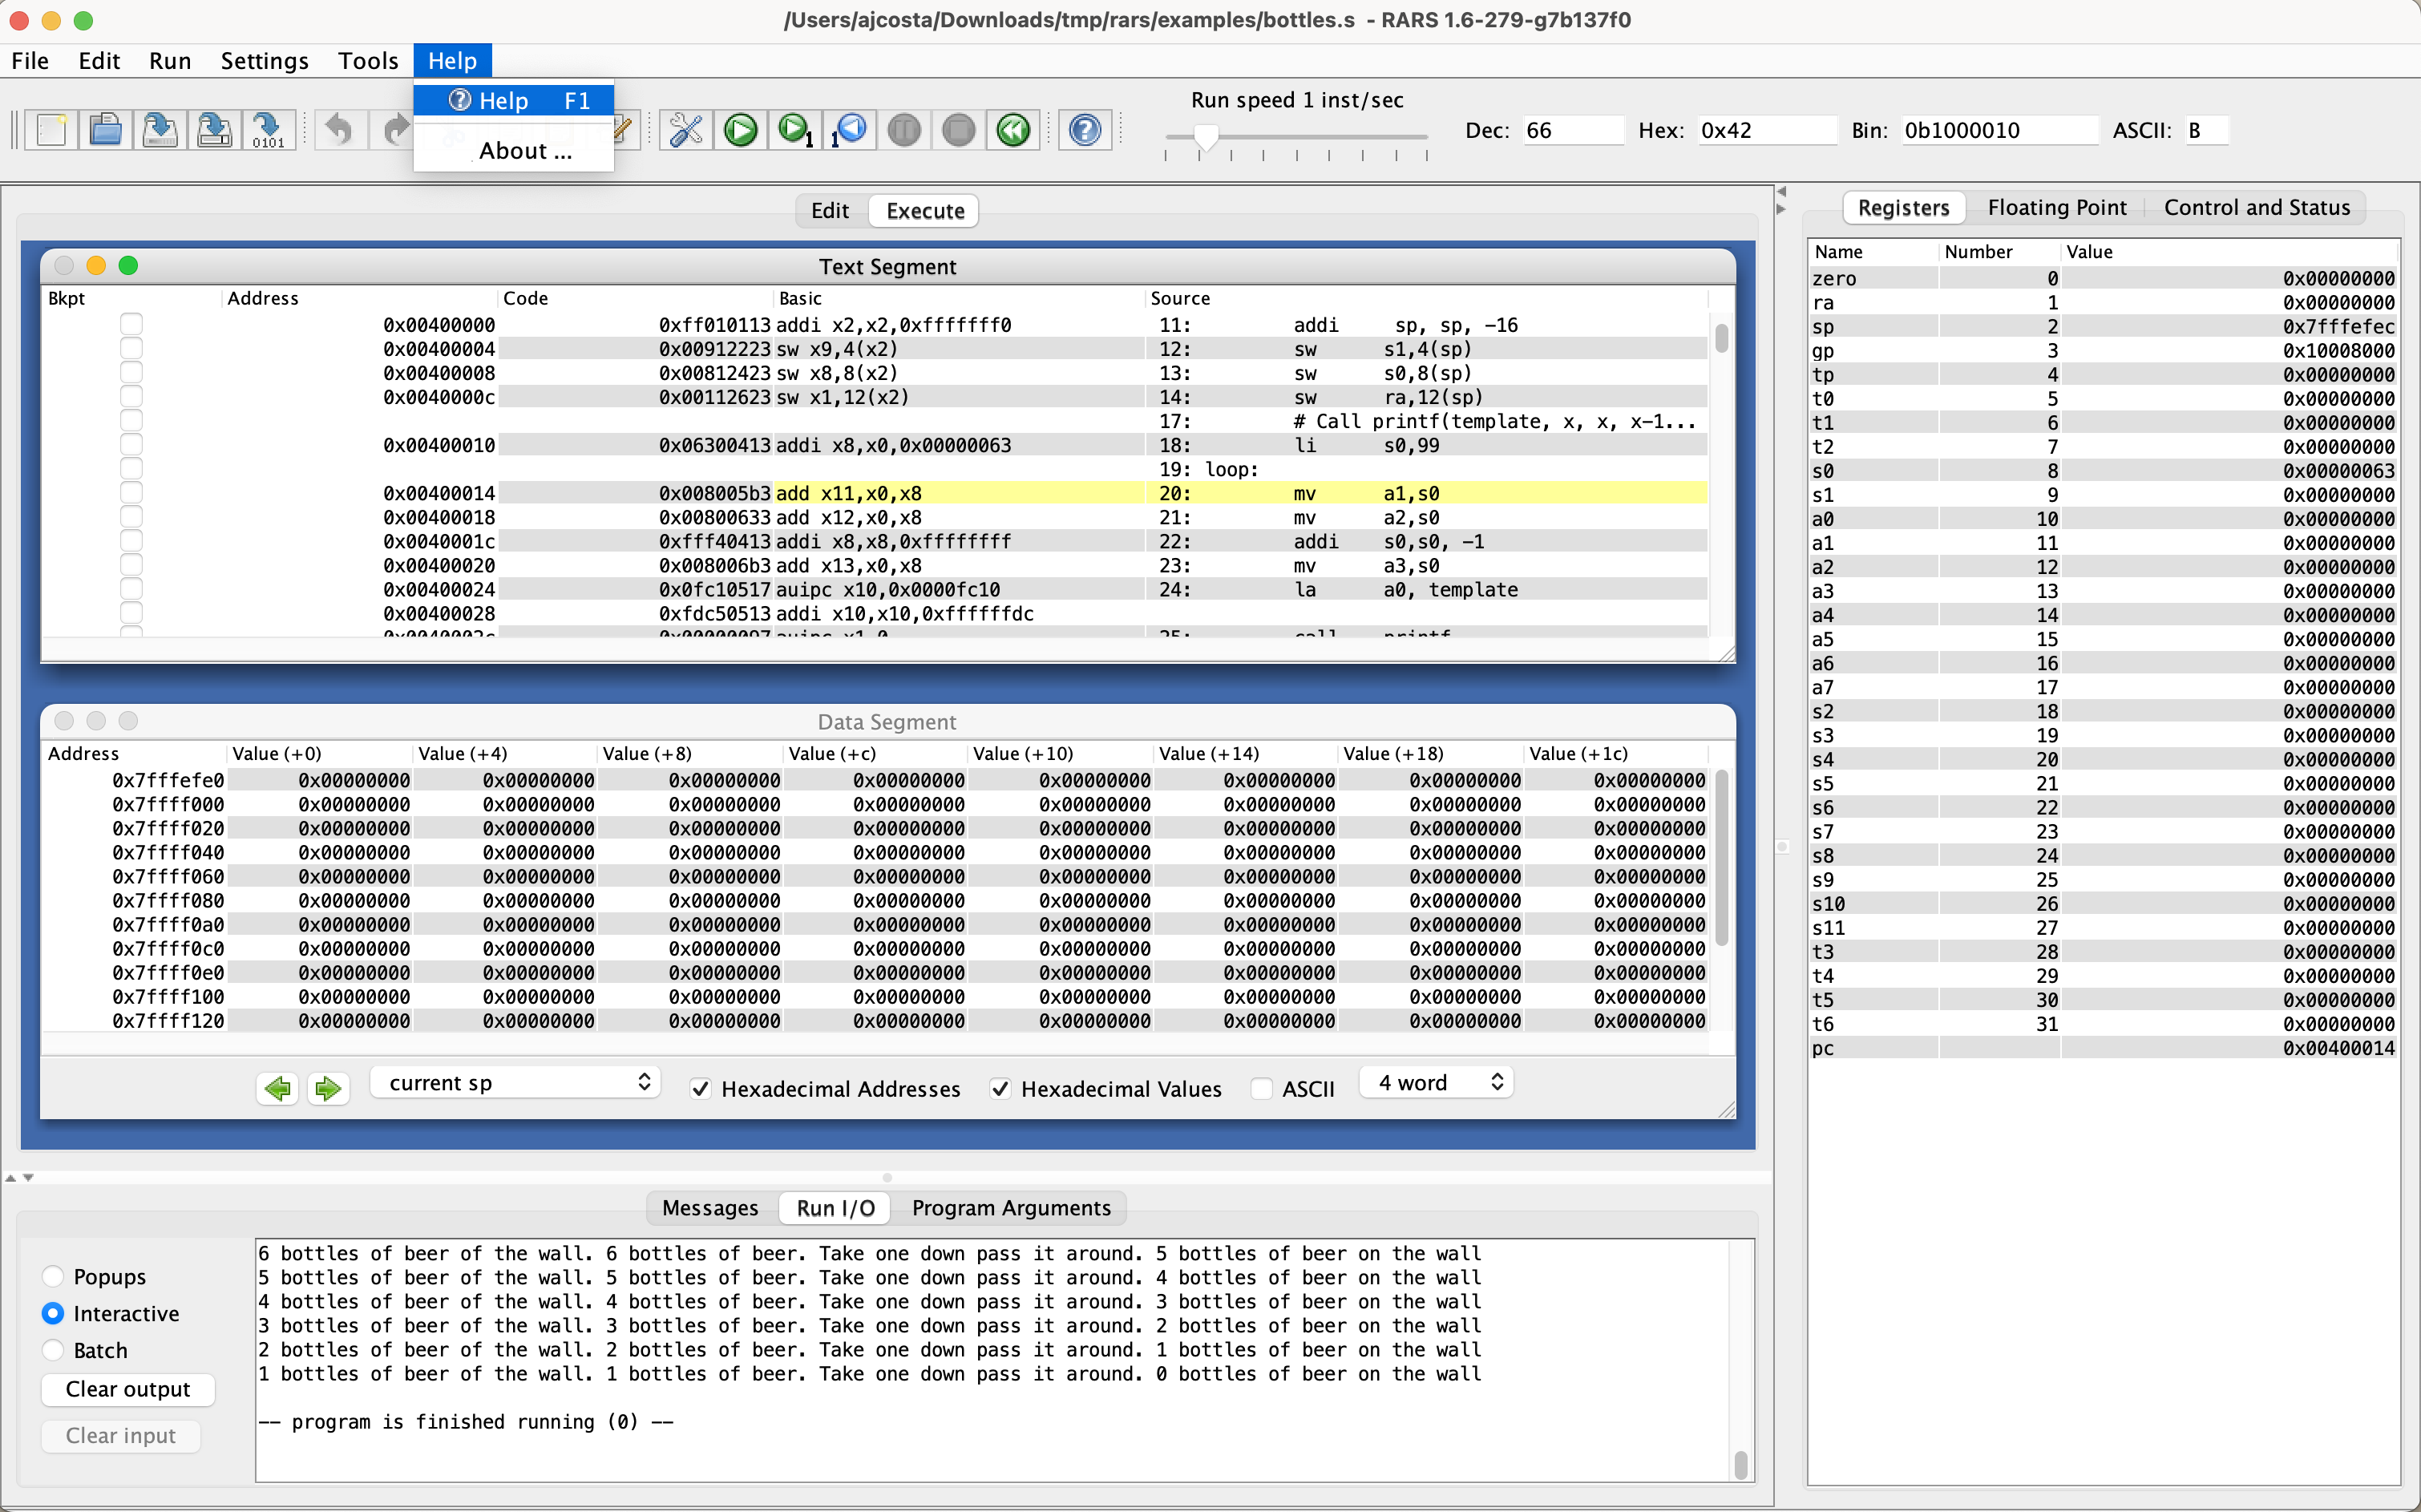
\includegraphics[width=0.85\paperwidth]{rsrcs/14_documentation.png}}
    %\caption{14: Documentation}
\end{figure}

You will reach this window, which shows you many RISC-V instructions, syscalls, and much more!

\begin{figure}[H]
    \centering
    \makebox[\textwidth]{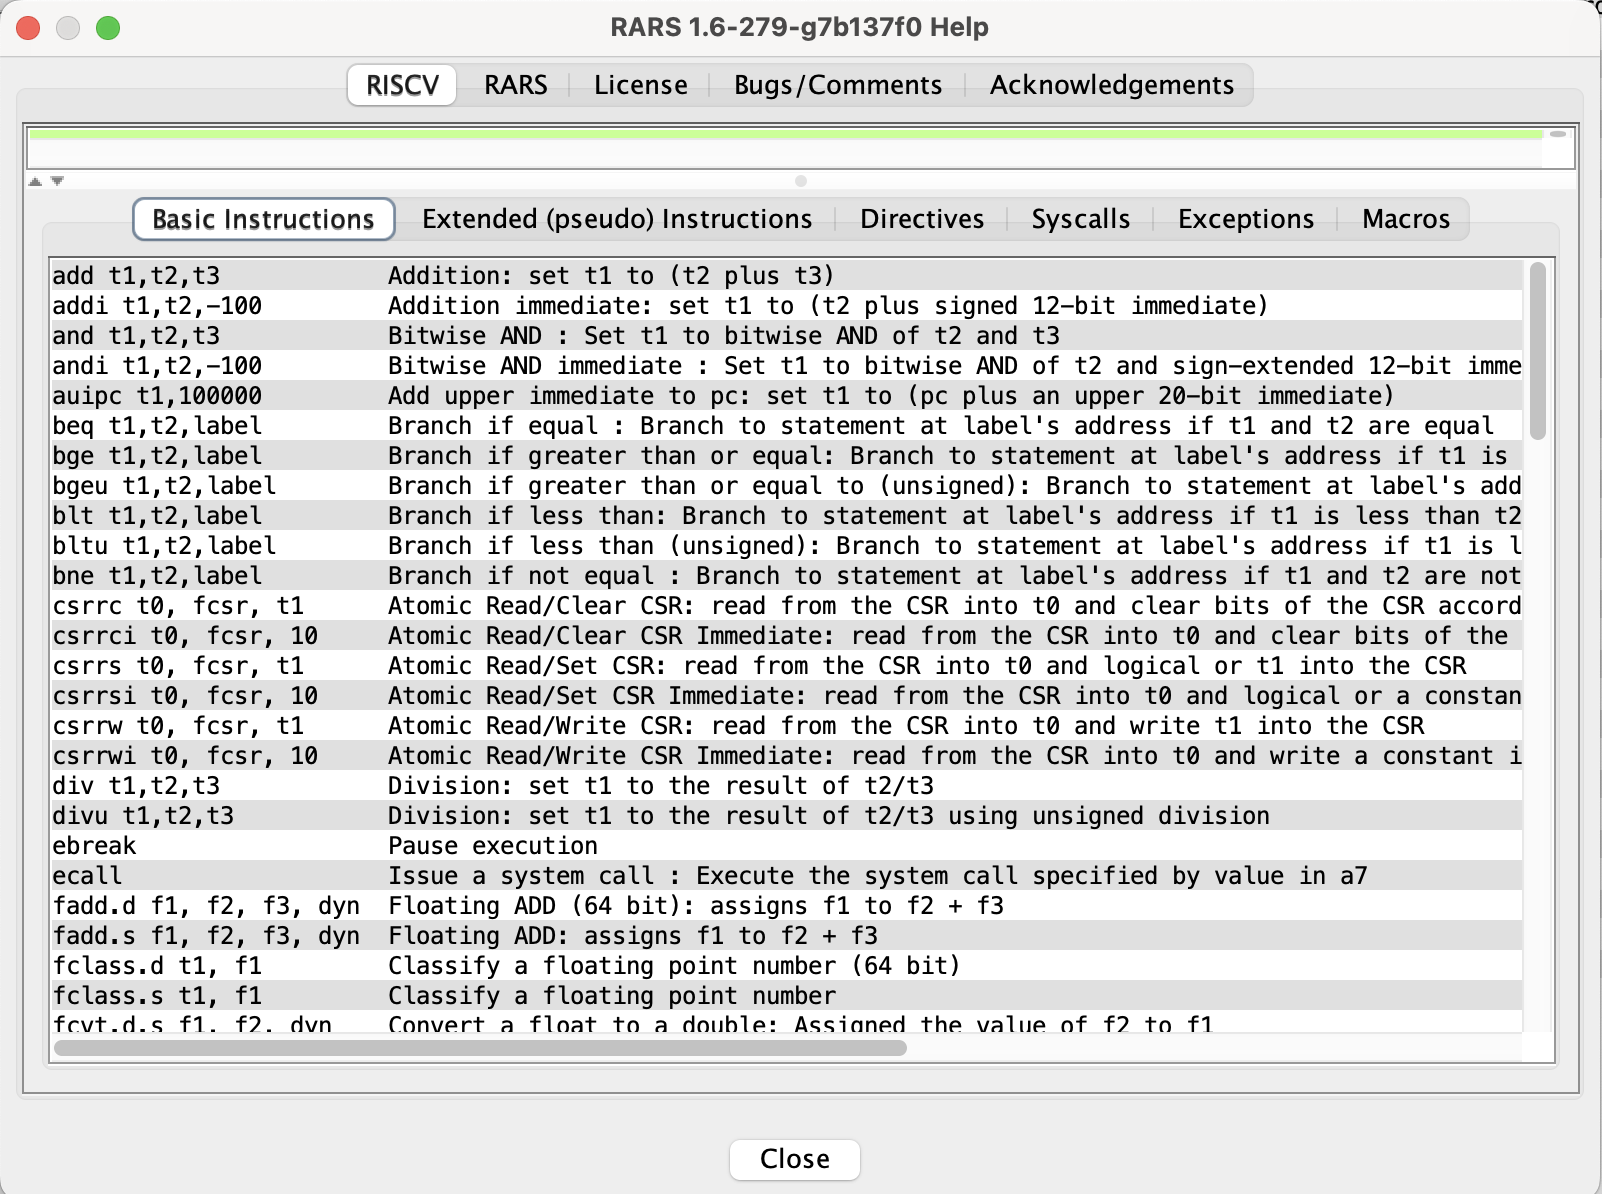
\includegraphics[width=0.75\paperwidth]{rsrcs/15_documentation.png}}
    %\caption{15: Documentation}
\end{figure}


Happy assembling :)!

\end{document}
